% ******************************* PhD Thesis Template **************************
% Please have a look at the README.md file for info on how to use the template

\documentclass[a4paper,12pt,times,numbered,print,custommargin,index,custombib,oneside]{Classes/PhDThesisPSnPDF}

\usepackage{tocloft}
\setlength\cftparskip{0pt}
\setlength\cftbeforechapskip{0pt}

% ******************************************************************************
% ******************************* Class Options ********************************
% *********************** See README for more details **************************
% ******************************************************************************

% `a4paper'(The University of Cambridge PhD thesis guidelines recommends a page
% size a4 - default option) or `a5paper': A5 Paper size is also allowed as per
% the Cambridge University Engineering Deparment guidelines for PhD thesis
%
% `11pt' or `12pt'(default): Font Size 10pt is NOT recommended by the University
% guidelines
%
% `oneside' or `twoside'(default): Printing double side (twoside) or single
% side.
%
% `print': Use `print' for print version with appropriate margins and page
% layout. Leaving the options field blank will activate Online version.
%
% `index': For index at the end of the thesis
%
% `draftclassic': For draft mode without loading any images (same as draft in book)
%
% `draft': Special draft mode with line numbers, images, and water mark with
% timestamp and custom text. Position of the text can also be modified.
%
% `abstract': To generate only the title page and abstract page with
% dissertation title and name, to submit to the Student Registry
%
% `chapter`: This option enables only the specified chapter and it's references
%  Useful for review and corrections.
%
% ************************* Custom Page Margins ********************************
%
% `custommargin`: Use `custommargin' in options to activate custom page margins,
% which can be defined in the preamble.tex. Custom margin will override
% print/online margin setup.
%
% *********************** Choosing the Fonts in Class Options ******************
%
% `times' : Times font with math support. (The Cambridge University guidelines
% recommend using times)
%
% `fourier': Utopia Font with Fourier Math font (Font has to be installed)
%            It's a free font.
%
% `customfont': Use `customfont' option in the document class and load the
% package in the preamble.tex
%
% default or leave empty: `Latin Modern' font will be loaded.
%
% ********************** Choosing the Bibliography style ***********************
%
% `authoryear': For author-year citation eg., Krishna (2013)
%
% `numbered': (Default Option) For numbered and sorted citation e.g., [1,5,2]
%
% `custombib': Define your own bibliography style in the `preamble.tex' file.
%              `\RequirePackage[square, sort, numbers, authoryear]{natbib}'.
%              This can be also used to load biblatex instead of natbib
%              (See Preamble)
%
% **************************** Choosing the Page Style *************************
%
% `default (leave empty)': For Page Numbers in Header (Left Even, Right Odd) and
% Chapter Name in Header (Right Even) and Section Name (Left Odd). Blank Footer.
%
% `PageStyleI': Chapter Name next & Page Number on Even Side (Left Even).
% Section Name & Page Number in Header on Odd Side (Right Odd). Footer is empty.
%
% `PageStyleII': Chapter Name on Even Side (Left Even) in Header. Section Number
% and Section Name in Header on Odd Side (Right Odd). Page numbering in footer

% Uncomment to change page style
%\pagestyle{PageStyleII}

% ********************************** Preamble **********************************
% Preamble: Contains packages and user-defined commands and settings
% ******************************************************************************
% ****************************** Custom Margin *********************************

% Add `custommargin' in the document class options to use this section
% Set {innerside margin / outerside margin / topmargin / bottom margin}  and
% other page dimensions
\ifsetCustomMargin
\RequirePackage[left=40mm,right=20mm,top=30mm,bottom=30mm]{geometry}
  \setFancyHdr % To apply fancy header after geometry package is loaded
\fi

% Add spaces between paragraphs
%\setlength{\parskip}{0.5em}
% Ragged bottom avoids extra whitespaces between paragraphs
\raggedbottom
% To remove the excess top spacing for enumeration, list and description
%\usepackage{enumitem}
%\setlist[enumerate,itemize,description]{topsep=0em}
\usepackage{bm}
\usepackage{mathtools}
\usepackage{amsmath} 
\usepackage{tikz}
\usepackage{pgfplots}
\usepackage{amsfonts}
\usepackage{amssymb}
\usepackage[makeroom]{cancel}
\usepackage{fancyhdr}
\usepackage{calligra}


% *****************************************************************************
% ******************* Fonts (like different typewriter fonts etc.)*************

% Add `customfont' in the document class option to use this section

\ifsetCustomFont
  % Set your custom font here and use `customfont' in options. Leave empty to
  % load computer modern font (default LaTeX font).
  %\RequirePackage{helvet}

  % For use with XeLaTeX
  %  \setmainfont[
  %    Path              = ./libertine/opentype/,
  %    Extension         = .otf,
  %    UprightFont = LinLibertine_R,
  %    BoldFont = LinLibertine_RZ, % Linux Libertine O Regular Semibold
  %    ItalicFont = LinLibertine_RI,
  %    BoldItalicFont = LinLibertine_RZI, % Linux Libertine O Regular Semibold Italic
  %  ]
  %  {libertine}
  %  % load font from system font
  %  \newfontfamily\libertinesystemfont{Linux Libertine O}
\fi

% *****************************************************************************
% **************************** Custom Packages ********************************

% ************************* Algorithms and Pseudocode **************************

%\usepackage{algpseudocode}


% ********************Captions and Hyperreferencing / URL **********************

% Captions: This makes captions of figures use a boldfaced small font.
%\RequirePackage[small,bf]{caption}

\RequirePackage[labelsep=space,tableposition=top]{caption}
\renewcommand{\figurename}{Fig.} %to support older versions of captions.sty


% *************************** Graphics and figures *****************************

%\usepackage{rotating}
%\usepackage{wrapfig}

% Uncomment the following two lines to force Latex to place the figure.
% Use [H] when including graphics. Note 'H' instead of 'h'
%\usepackage{float}
%\restylefloat{figure}

% Subcaption package is also available in the sty folder you can use that by
% uncommenting the following line
% This is for people stuck with older versions of texlive
%\usepackage{sty/caption/subcaption}
\usepackage{subcaption}

% ********************************** Tables ************************************
\usepackage{booktabs} % For professional looking tables
\usepackage{multirow}

\usepackage{multicol}
%\usepackage{longtable}
%\usepackage{tabularx}
%\usepackage[spanish]{babel}

% *********************************** SI Units *********************************
\usepackage{siunitx} % use this package module for SI units


% ******************************* Line Spacing *********************************

% Choose linespacing as appropriate. Default is one-half line spacing as per the
% University guidelines

% \doublespacing
% \onehalfspacing
% \singlespacing

\usepackage{hhline}
% ************************ Formatting / Footnote *******************************

% Don't break enumeration (etc.) across pages in an ugly manner (default 10000)
%\clubpenalty=500
%\widowpenalty=500

%\usepackage[perpage]{footmisc} %Range of footnote options


% *****************************************************************************
% *************************** Bibliography  and References ********************

%\usepackage{cleveref} %Referencing without need to explicitly state fig /table

% Add `custombib' in the document class option to use this section
\ifuseCustomBib
   \RequirePackage[square, sort, numbers, authoryear]{natbib} % CustomBib

% If you would like to use biblatex for your reference management, as opposed to the default `natbibpackage` pass the option `custombib` in the document class. Comment out the previous line to make sure you don't load the natbib package. Uncomment the following lines and specify the location of references.bib file

%\RequirePackage[backend=biber, style=numeric-comp, citestyle=numeric, sorting=nty, natbib=true]{biblatex}
%\addbibresource{References/references} %Location of references.bib only for biblatex, Do not omit the .bib extension from the filename.

\fi

% changes the default name `Bibliography` -> `References'
\renewcommand{\bibname}{References}


% ******************************************************************************
% ************************* User Defined Commands ******************************
% ******************************************************************************

% *********** To change the name of Table of Contents / LOF and LOT ************

%\renewcommand{\contentsname}{My Table of Contents}
%\renewcommand{\listfigurename}{My List of Figures}
%\renewcommand{\listtablename}{My List of Tables}


% ********************** TOC depth and numbering depth *************************

\setcounter{secnumdepth}{2}
\setcounter{tocdepth}{2}


% ******************************* Nomenclature *********************************

% To change the name of the Nomenclature section, uncomment the following line

%\renewcommand{\nomname}{Symbols}


% ********************************* Appendix ***********************************

% The default value of both \appendixtocname and \appendixpagename is `Appendices'. These names can all be changed via:

%\renewcommand{\appendixtocname}{List of appendices}
%\renewcommand{\appendixname}{Appndx}

% *********************** Configure Draft Mode **********************************

% Uncomment to disable figures in `draft'
%\setkeys{Gin}{draft=true}  % set draft to false to enable figures in `draft'

% These options are active only during the draft mode
% Default text is "Draft"
%\SetDraftText{DRAFT}

% Default Watermark location is top. Location (top/bottom)
%\SetDraftWMPosition{bottom}

% Draft Version - default is v1.0
%\SetDraftVersion{v1.1}

% Draft Text grayscale value (should be between 0-black and 1-white)
% Default value is 0.75
%\SetDraftGrayScale{0.8}
%\newenvironment{poliabstract}[1]
%{\renewcommand{\abstractname}{#1}\begin{abstract}}
%	{\end{abstract}}


% ******************************** Todo Notes **********************************
%% Uncomment the following lines to have todonotes.

%\ifsetDraft
%	\usepackage[colorinlistoftodos]{todonotes}
%	\newcommand{\mynote}[1]{\todo[author=kks32,size=\small,inline,color=green!40]{#1}}
%\else
%	\newcommand{\mynote}[1]{}
%	\newcommand{\listoftodos}{}
%\fi

% Example todo: \mynote{Hey! I have a note}

% ******************************** Highlighting Changes **********************************
%% Uncomment the following lines to be able to highlight text/modifications.
%\ifsetDraft
%  \usepackage{color, soul}
%  \newcommand{\hlc}[2][yellow]{{\sethlcolor{#1} \hl{#2}}}
%  \newcommand{\hlfix}[2]{\texthl{#1}\todo{#2}}
%\else
%  \newcommand{\hlc}[2]{}
%  \newcommand{\hlfix}[2]{}
%\fi

% Example highlight 1: \hlc{Text to be highlighted}
% Example highlight 2: \hlc[green]{Text to be highlighted in green colour}
% Example highlight 3: \hlfix{Original Text}{Fixed Text}

% *****************************************************************************
% ******************* Better enumeration my MB*************
\usepackage{enumitem}

% ************************ Thesis Information & Meta-data **********************
%% The title of the thesis
\title{\Large Study of the production of Higgs plus single top using events with a same sign dimuon pair in the final state at the Large Hadron Collider}
%\texorpdfstring is used for PDF metadata. Usage:
%\texorpdfstring{LaTeX_Version}{PDF Version (non-latex)} eg.,
%\texorpdfstring{$sigma$}{sigma}

%% Subtitle (Optional)
%\subtitle{Using the CUED template}

%% The full name of the author
\author{Hiram Ernesto Dami\'an}

%% Department (eg. Department of Engineering, Maths, Physics)
\dept{Departmento de Investigaci\'on en F\'isica}

%% University and Crest
\university{Universidad de Sonora\\
Divisi\'on de Ciencias Exactas y Naturales}
% Crest minimum should be 30mm.
\crest{
\includegraphics[width=0.4\textwidth]{unison-logo.png}}
%% Use this crest, if you are using the college crest
%% Crest long miminum should be 65mm
%\crest{
\includegraphics[width=0.45\textwidth]{University_Crest_Long}}

%% College shield [optional] 
% Crest minimum should be 30mm.
%\collegeshield{
\includegraphics[width=0.2\textwidth]{CollegeShields/Kings}}


%% Supervisor (optional)
%% for multiple supervisors, append each supervisor with the \newline command

\supervisor{Jos\'e Feliciano Ben\'itez Rubio}
%Prof. C.D. Supervisor}

%% Supervisor Role (optional) - Supervisor (default) or advisor
% \supervisorrole{\textbf{Supervisors: }}
%\supervisorrole{Jos\'e Feliciano Ben\'itez Rubio}
%% if no title is desired:
% \supervisorrole{}

%% Supervisor line width: required to align supervisors
%\supervisorlinewidth{0.35\textwidth}

%% Advisor (optional)
%% for multiple advisors, append each advisor with the \newline command
%\advisor{Dr. A. Advisor\newline
%Dr. B. Advisor}
     
%% Advisor Role (optional) - Advisor (default) or leave empty
% \advisorrole{Advisors: }
%% if no title is required
% \advisorrole{}

%% Advisor line width: required to align supervisors
%\advisorlinewidth{0.25\textwidth}


%% You can redefine the submission text:
% Default as per the University guidelines:
% ``This dissertation is submitted for the degree of''
\renewcommand{\submissiontext}{Tesis para obtener el grado de:\\
\textbf{Maestr\'ia en Ciencias (F\'isica)}}

%% Full title of the Degree
%\degreetitle{Doctor of Philosophy}

%% College affiliation (optional)
\college{Hermosillo, Sonora}

%% Submission date
% Default is set as {\monthname[\the\month]\space\the\year}
%\degreedate{September 2014} 

%% Meta information
\subject{LaTeX} \keywords{{LaTeX} {PhD Thesis} {Engineering} {University of
Cambridge}}

% ************************ Thesis Information & Meta-data **********************
% Thesis title and author information, refernce file for biblatex

% ***************************** Abstract Separate ******************************
% To printout only the titlepage and the abstract with the PhD title and the
% author name for submission to the Student Registry, use the `abstract' option in
% the document class.


\ifdefineAbstract
\pagestyle{empty}
\includeonly{Declaration/declaration, Abstract/abstract, Abstract/resumen}
\fi

% ***************************** Chapter Mode ***********************************
% The chapter mode allows user to only print particular chapters with references
% Title, Contents, Frontmatter are disabled by default
% Useful option to review a particular chapter or to send it to supervisior.
% To use choose `chapter' option in the document class

\ifdefineChapter
\includeonly{Chapter3/chapter3}
\fi

% ******************************** Front Matter ********************************
\begin{document}
	
	\frontmatter
	\maketitle
	
	% ******************************* Thesis Dedidcation *******************************
\begin{dedication} 
I would like to dedicate this thesis to my loving mother \dots
\end{dedication}
	%% ******************************* Thesis Declaration ***************************

\begin{declaration}

I hereby declare that except where specific reference is made to the work of 
others, the contents of this dissertation are original and have not been 
submitted in whole or in part for consideration for any other degree or 
qualification in this, or any other university. This dissertation is my own 
work and contains nothing which is the outcome of work done in collaboration 
with others, except as specified in the text and Acknowledgements. This 
dissertation contains fewer than 65,000 words including appendices, 
bibliography, footnotes, tables and equations and has fewer than 150 figures.

% Author and date will be inserted automatically from thesis.tex \author \degreedate

\end{declaration}
	% ************************** Thesis Acknowledgements **************************

\begin{acknowledgements}      
 I would like to acknowledge Dr. Jos\'e Feliciano Ben\'itez Rubio for his contributions and advises in order to develop  and write this thesis. Also thank Dr. Javier Murillo and  Dr. Cristina Oropeza for their observations and advises in my formation. 
Dr. Susana Alv\'arez for supporting during the process of the thesis. Acknowledgments to CONACYT for supporting this thesis with financial aid. 
\end{acknowledgements}

	
\thispagestyle{empty}
 \vspace*{2.2cm}
\begin{center}
\Large \textbf{Resumen}
\end{center} 
\vspace{1.5cm}

%\renewcommand{\absnamepos}{empty} % originally center
%\begin{center}
%	\justifying
Se presenta un estudio sobre la producci\'on del boson de Higgs y un top quark ($tH$) en el canal de 2 muones con el mismo signo $\mu^\pm \mu^\pm$ usando datos publicados por el experimento CMS en el CERN.
Estudiando este proceso se explora este mecanismo de producci\'on del boson de Higgs que a\'un no se ha detectado experimentalmente.
La sensibilidad esperada es calculada usando  datos de tipo Asimov para 35.9 fb$^{-1}$ de colisiones de prot\'on-prot\'on y es extrapolada la fase de alta luminosidad del LHC (HL-LHC).
La sensibilidad de la se\~nal es tambi\'en estudiada para el modelo con acoplamiento de Yukawa invertido $k_t$=-1, donde $k_t$ es el modificador del par\'ametro de acoplamiento de top-Higgs, en comparaci\'on con el Modelo Est\'andar.
%\end{center}

	\thispagestyle{empty}
\vspace*{2.2cm}
\begin{center}
	\Large \textbf{Abstract}
\end{center} 
\vspace{1.5cm}


% ************************** Thesis Abstract *****************************
% Use `abstract' as an option in the document class to print only the titlepage and the abstract.
%\begin{center}
%	\justifying
I present a study on the production of a Higgs boson plus a single top quark ($tH$) in same sign dimuon channel $\mu^\pm \mu^\pm$ using data published by the CMS experiment at CERN. By studying this
process I explore a Higgs production mechanism which has not yet been observed
experimentally. The expected sensitivity is estimated by using an Asimov dataset for 35.9 fb$^{-1}$ of proton-proton collisions and is extrapolated to the  high luminosity phase of the LHC (HL-LHC).
The sensivity is also studied for the model with inverted Yukawa coupling $k_t$=-1, where $k_t$ is the top-Higgs coupling parameter modifier, for comparison with the Standard Model.
%\end{center}

	% *********************** Adding TOC and List of Figures ***********************
	
	\tableofcontents
	\pagebreak
	\listoffigures
	\pagebreak
	\listoftables
	\pagebreak
	% \printnomenclature[space] space can be set as 2em between symbol and description
	%\printnomenclature[3em]
	
	\printnomenclature
	
	% ******************************** Main Matter *********************************
	\mainmatter
	
		%!TEX root =../thesis.tex
%*******************************************************************************
%*********************************** First Chapter *****************************
%*******************************************************************************
%\renewcommand{\baselinestretch}{1.5}

\begin{chapter}{Introduction}

\section{General objective and motivations}

Particle physics is a field of physics that studies the particles that create matter and their interactions to very small scale, even smaller than atoms. 
Particle physics studies the fundamental building blocks of matter (fermions) and their interactions via force carriers (bosons). 
%The particles analyzed in particle physics are the fundamental particles that compose matter and the responsible for all forces of nature.
All those particles and their properties are grouped in a theory called the Standard Model (SM). SM is a theory that describes the fundamental forces (except gravity) and classifies the elementary particles in bosons (integer spin) and fermions (half spin).
The SM, created almost 50 years ago, has been the most successful theory in explaining the phenomena in the subatomic world.

One of the particles of the SM, the Higgs Boson, was recently discovered in 2012 in the ATLAS and CMS experiments at CERN. The discovery of Higgs boson in proton proton (pp) collisions marked a new era in particle physics due to its characteristic of giving matter the property of mass, according to previous theories and predictions. Since then, people around the world are working in the Large Hadron Collider (LHC) at CERN in order to detect the Higgs bosons in higher energies and different Higgs production processes. 
Also the Higgs boson is also important in cosmology, where theoretical investigations relate the Higgs boson to the cosmic inflation.

In recent years, there have been many studies of Higgs production processes at CERN in pp collisions, such as gluon fusion (ggF), VBF, WH, ZH and $t\bar{t}H$. 
In this work, we will analyze the production of a Higgs boson in association with a
single top quark (tH) in pp collisions with the CMS experiment of the LHC. 

The motivation of the work is that this production mechanism of the Higgs boson has not been observed before by any experiment. The exploration of Higgs production on the tH channel is a relatively new subject. %The SM is used to study the tH channel and compare it with other Higgs production mechanisms results.
Many channels are yet out of
reach experimentally. At the same time, many theoretical
proposals are yet to be put to test. It is possible that studies on the Higgs boson give evidence of small deviations from the SM and test new physics that are beyond SM such as String Theory and Super-symmetry. 

%********************************** % Third Section *************************************
\section{The Standard Model} %Section - 1.3 
The SM, created in the decade of the seventies, is a successful theory that explains the structure of matter and the interactions of three of the four fundamental forces which are electromagnetic, strong and weak. The gravitational force is yet to be included due to the scale of the interaction with respect to the other 3. All matter is composed of three kinds of particles: leptons, quarks and bosons, also called mediators.

For the leptons we have electrons ($e$), muons ($\mu$), and taus ($\tau$) with charge -1 and their neutrinos $\nu_e, \nu_\mu, \nu_\tau$, are chargeless particles. %Leptons have their respective antiparticle; same structure with opposite charge. 
 All of them have a spin (intrinsic angular momentum) of $\frac{1}{2}$\cite{griff}. % In case of neutrinos, so far experimentalists have found these have very small masses, but in the theoretical scheme, they are massless. \\
 Quarks combine to form composite particles called hadrons. Quarks cannot be found in isolation, they always exist in form of hadrons that can be mesons or baryons. Mesons are made up of a quark-antiquark pair, such as pion ($\pi$) and kaon ($K$). Mesons were theorized by Yukawa in 1937 and discovered in 1947 by Powell\cite{griff}.
Baryons are made of 3 quarks. Examples of baryons are protons and neutrons. Both types of particles can interact via the strong force. Since quarks and gluons only exist in bound, it is impossible to observe isolated quarks except the top quark, which decays before it has time to form a
bound state \cite{gross}.

Quarks were first theorized by Murray Gell-Mann and 
George Zweig in 1964. They were introduced as parts of an ordering scheme for hadrons, and there was little evidence for their physical existence until fixed target scattering experiments were conducted at the Stanford Linear Accelerator Center in 1968\cite{griff}.
There are 6 of them: up (1968), down (1968), strange (1968), charm (theorized in 1970, discovered 1974), bottom (theorized 1973, discovered 1977), top (theorized 1973, discovered 1995).

Quarks have characteristics such as electric charge, mass, color charge, and spin. The quarks up, charm and top have in common a charge of $\frac{2}{3}$, while the down, strange and bottom quarks have charge of $-\frac{1}{3}$. Among them, the top quark is the most massive of all, while the up and down are the least massive. 
Some of the particles in the SM are not stable, so they decays and form particles with lower masses. Other particles do not decay or their lifetimes are very long. All the particles in the SM are shown in the figure \ref{sm1}. %The final states can be represented with a Feynman diagram according to the SM vertices\cite{mark}.

\begin{center}
  \begin{figure}[ht]
    \centering
    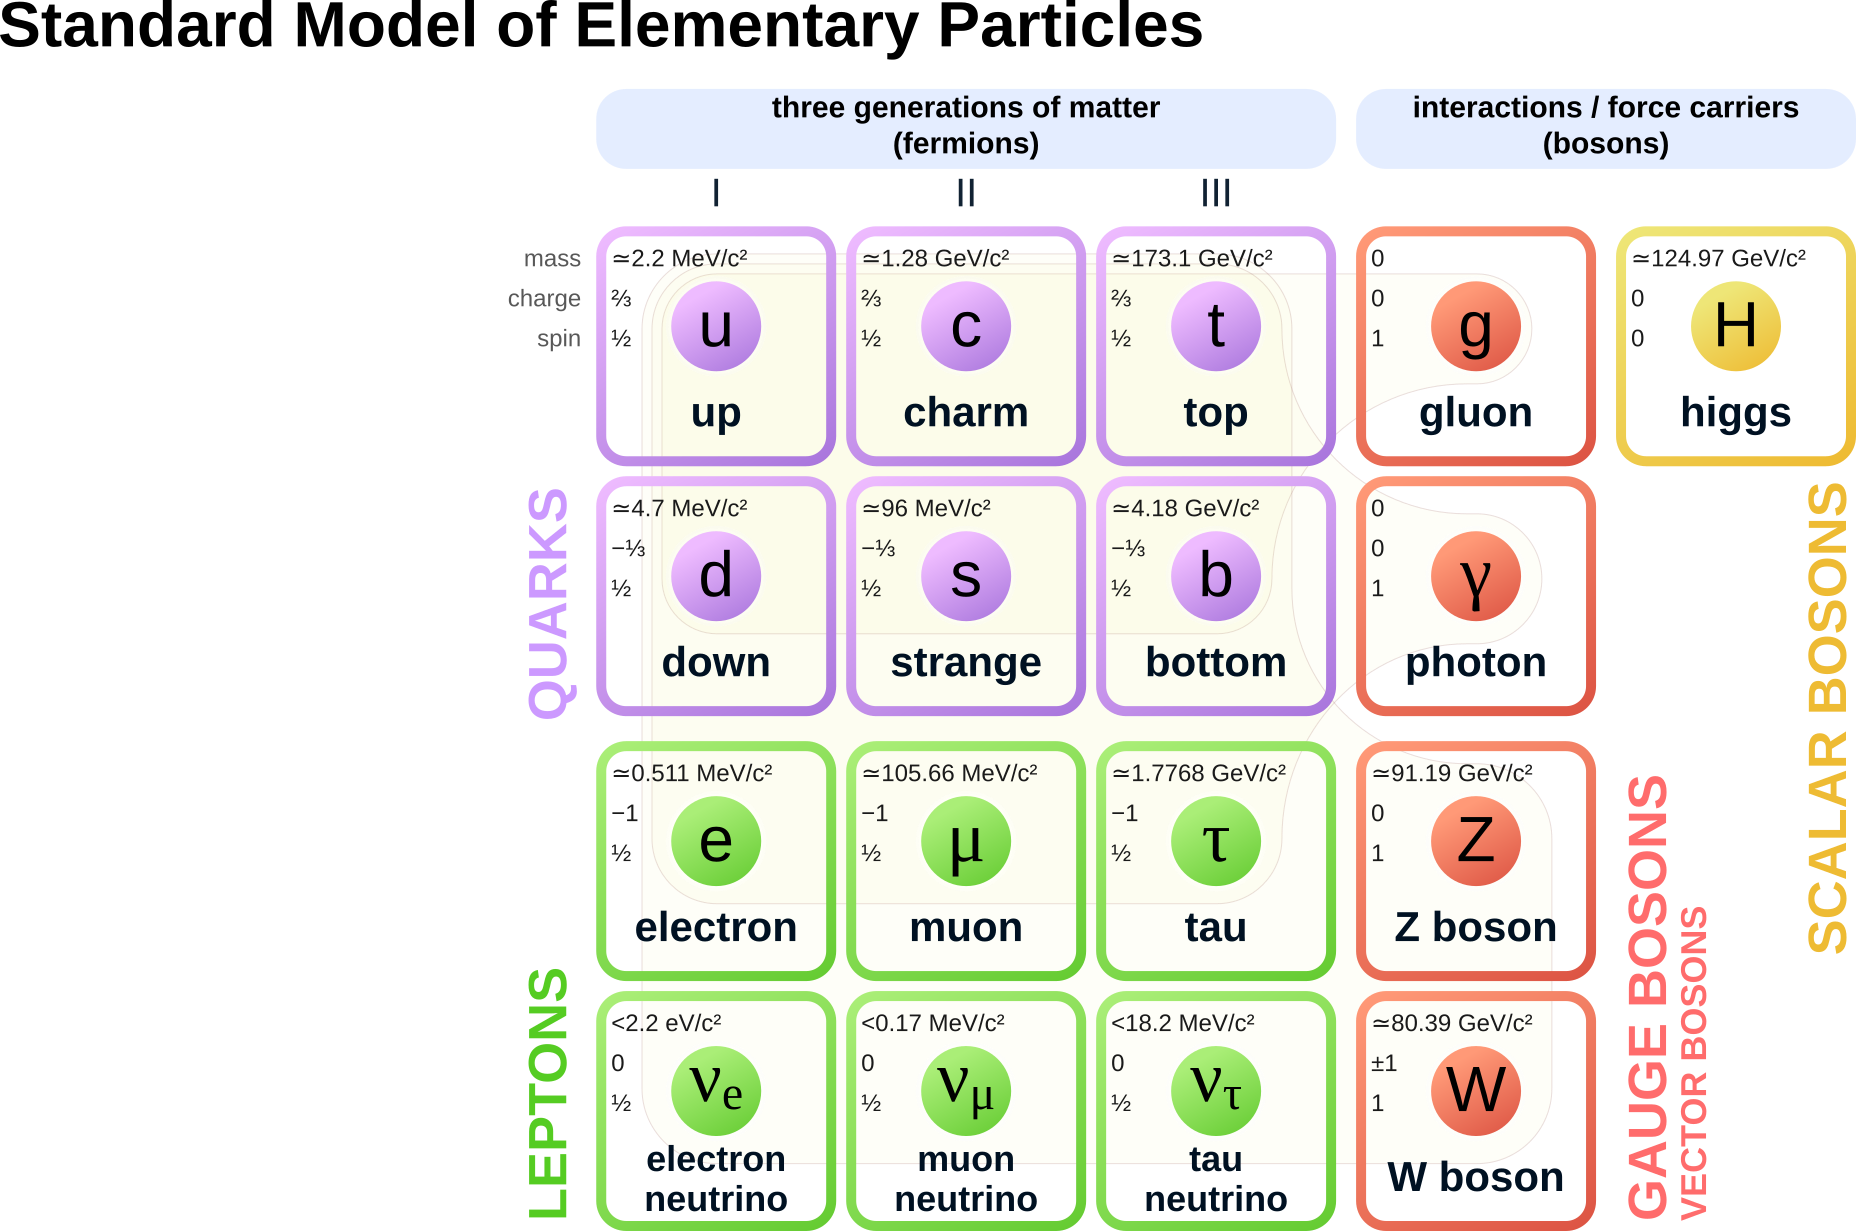
\includegraphics[scale=0.3]{Chapter1/sm1.png}
    \caption[Standard Model to date]{Standard Model to date\cite{smtable}}
    \label{sm1}
  \end{figure}
\end{center}
The last group of the family are the bosons, which have either spin 1 or 0. 
There are 5 bosons: $W^{\pm}$, $Z$ with neutral charge are responsible for weak force; photon, a massless particle, is responsible for the electromagnetic force; gluons which are also massless, is related to the strong force and Higgs boson, recently discovered, is in charge of giving the property of mass to particles via the Higgs mechanism. Bosons let other particles interact, even themselves, which is shown in Figure \ref{sm}. 
The $W$,$Z$ and Higgs bosons, can interact with the most of the particles, while the gluons can only interact with quarks and with itself.
%Those bosons act as mediators in decays and creation of complex
%particles, as mesons and baryons.

%In case of gravity, exist a theoretical particle, called graviton, that is the fundamental particle associated with the gravitational force. In case of its existance, it should have a spin 2 and mass 0. 

%There are experiments that detect particles around the world, such as the LHC in Europe, the Fermilab in United States of America, KEK in Japan, etc. More information about the LHC will be described in the next chapters. 

	\begin{figure}[ht]
		\centering
		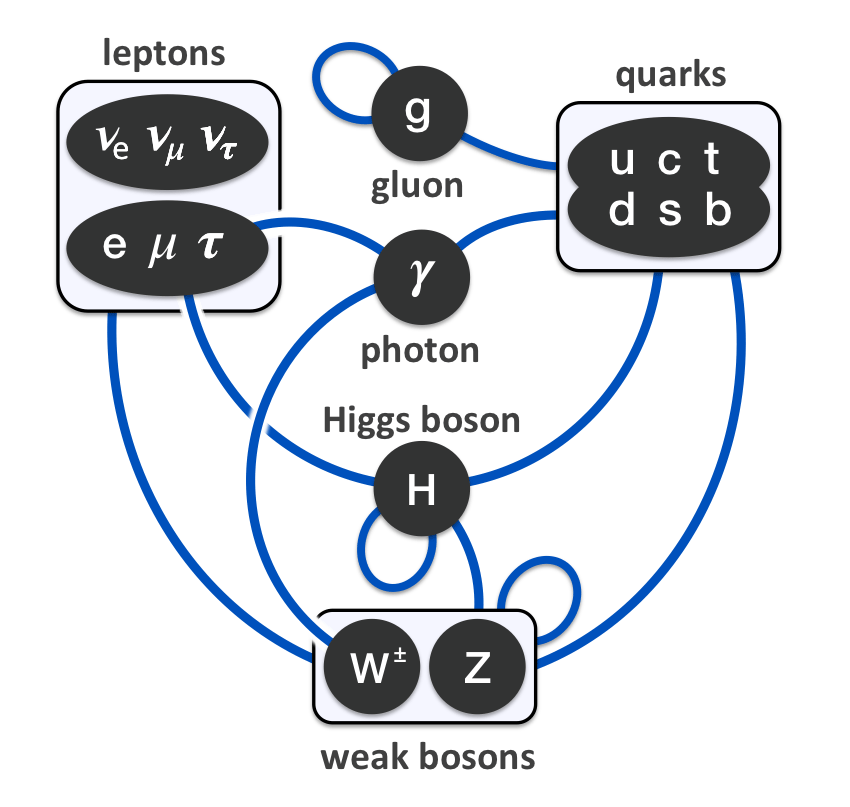
\includegraphics[scale=0.35]{Chapter1/sm.png}
		\caption[Particle interactions in Standard model]{Particle interactions in Standard model\cite{smi}}
		\label{sm}
	\end{figure}

Table \ref{SM table} contains the characteristics of each particle in the SM. The second column shows the masses of the particles, where the most massive particle is the top quark with 173 GeV. There are particles with mass equal to zero, such as the gluons, photons and the neutrinos. 
The third column corresponds to the charge of the particles. For the quarks, there are two different charges: $\frac{2}{3}$ for $u$,$c$ and $t$ and $-\frac{1}{3}$ for $d$,$s$ and $b$. For the leptons, the charge is negative, except for neutrinos, which charge is zero. 
The bosons have a integer charge; $\pm 1$ for $W$ and 0 for $Z$, $\gamma$, $H$ and $g$.	
The next column is the spin, where for fermions (quarks and leptons) is $\frac{1}{2}$ and for bosons is 1\footnote{In general, the fermions have non integer spin and the bosons have integer spin}. The Higgs boson is the only boson with spin 0.
The next one is the lifetime of the particle, where it shows how long the particles exist before decay. Stable lifetime means that the particles do not decay or lifetime almost infinite.
The last column is the distance of particles moving with speeds near light speed. This column illustrates the distance traveled in the predicted lifetime of the particle. And also give us a perspective of how hard the detection of  particles due to their lifetime is.  

\begin{table}[htp]
\caption[Table of particles in SM]{SM particle properties: mass, charges, spin, lifetime and distance traveled in a lifetime (assuming speed of $v$=0.998c)\cite{pd}. In the case of $s$,$c$ and $b$ quarks, the lifetime corresponds to the K$^\pm$, D$^{\pm}$ and B$^{\pm}$ meson lifetime.}
\renewcommand{\arraystretch}{1.5}
\begin{tabular}{|c|c|c|c|p{2.5cm}|p{2.5cm}|}
\hline 
Particle& Mass (MeV/$c^2$) &Charge & spin &Lifetime (s) & Distance (m) \\ 
	\hline 
Up quark ($u$)	& 2.2 & $\frac{2}{3}$ & $\frac{1}{2}$ & Stable & -\\ 
	\hline 
Charm quark ($c$)	& 1280 &$\frac{2}{3}$ & $\frac{1}{2}$ & $ 1.1 \times 10^{-12}$ & 5.21$\times 10^{-3}$ \\ 
	\hline 
Top	quark ($t$)& 173100 & $\frac{2}{3}$ & $\frac{1}{2}$ & 5$\times$10$^{-25}$ &2.37$\times 10^{-15}$  \\ 
	\hline 
Down quark ($d$)	& 4.6 &$-\frac{1}{3}$ & $\frac{1}{2}$ & Stable & - \\ 
	\hline 
Strange quark ($s$)	& 96 &$-\frac{1}{3}$ & $\frac{1}{2}$ &$1.2 \times 10^{-8}$ & 58.7 \\ 
	\hline 
Bottom quark ($b$)	& 4180 &$-\frac{1}{3}$ & $\frac{1}{2}$ &$1.6 \times 10^{-12}$  & 6.16 $\times 10^{-3}$\\ 
	\hline 
$W$ 	& 80379 &$\pm$1 & 1 & 3$\times$ 10$^{-25}$ & 1.4$\times 10^{-15}$\\ 
	\hline 
$Z$ & 91187.6 &0 & 1 & 3$\times$ 10$^{-25}$ &1.4$\times 10^{-15}$ \\ 
\hline
Photon ($\gamma$) & 0 &0 & 1&Stable & - \\ 
\hline
Gluon ($g$)	& 0 &0 & 1&Stable & - \\ 
	\hline 
Higgs ($H$)	& 125.18 &0 & 0& 1.5 $\times$ $10^{-22}$ & 7.39$\times 10^{-13}$ \\ 
	\hline 
Electron ($e$)& 0.511 & -1 &  $\frac{1}{2}$& Stable & - \\ 
	\hline 
Muon ($\mu$)	& 105.7 & -1 & $\frac{1}{2}$ & 2.2$\times$10$^{-6}$ & 10419.85 \\ 
	\hline 
Tau ($\tau$)	& 1776.86 &-1 & $\frac{1}{2}$ & 2.9$\times$10$^{-13}$ & 1.37$\times 10^{-3}$\\ 
	\hline 
$\nu_e$, $\nu_\mu$, $\nu_\tau$&  $<$ 2.0 $\times$ 10$^{-6}$ & 0 & $\frac{1}{2}$ & Stable & -\\
	\hline 
\end{tabular} 
\label{SM table}
\end{table}

\newpage

\section{Higgs Boson}
The Higgs is a boson with spin 0 and chargeless. First theorized in 1964 by a group of theoretical physicist composed by Peter Higgs, Fran\c cois Englert, Robert Brout, Gerald Guralnik, C. Richard Hagen, and Tom Kibble in separate groups. They formulated the Higgs mechanism that explains the generation of mass for the fermions and massive bosons. 
The Higgs boson was discovered recently in year 2012 in the experiments ATLAS and CMS at CERN. The experiment was conducted using proton-proton collisions with center of mass energy of 7 and 8 TeV, where investigators analyzed the data in the $\gamma \gamma$ and $ZZ$ final states\cite{higgsd,Aad_2012}. 
The mass of this boson has been measured and its production and decay
rates are consistent with the SM prediction. The mass of the Higgs boson measured is 125.18 $\pm$ 0.16 GeV\cite{pd}. The Higgs boson lifetime is 1.56 $\times$ $10^{-22}$ s. That is why the Higgs boson was very difficult to detect in particle detectors. 

\section{Top quark}
The top quark is the most massive particle with a charge of 2/3 and spin of 1/2. First proposed by M. Kobayashi and T. Maskawa in 1973 to explain observed CP violations in Kaon decay\cite{griff}. In 1995, in the Tevatron at Fermilab in Illinois, the top quark was discovered via proton antiproton collisions with center of mass energy between 1.8 to 1.96 TeV in the CDF and D0 experiments. The top quark production process was via ggF, which generated a pair of $t\bar{t}$\cite{top}.
Since then, the properties of the top quark have been studied at the Tevatron Collider at Fermilab, and by the ATLAS and CMS experiments at the Large Hadron Collider (LHC) at CERN.
However, the top quark often receives special attention in new physics models because its mass requires near unity coupling to the Higgs boson\cite{top}.
As shown in Table \ref{SM table}, the top quark lifetime is so small that they decay before they can hadronise, that is to say, the process to create hadrons from quarks and gluons.

One of the interesting properties of top quark is its mass.
The top quark mass is a free parameter in the SM and was extracted using indirect measurements and relying on SM calculations. The measured value of the top quark mass is of 173 Gev\cite{pd}. The top quark mass is a very important
parameter that puts a constraint in the Higgs boson mass and also takes an important role in electroweak symmetry breaking\cite{top}.

The production of top quark can be generated in different ways. In Tevatron and LHC, the production of $t\bar{t}$ comes mainly from ggF (gluon gluon fusion) via strong force. Even it is possible to create a single top quark in the LHC via electroweak interactions (with a W boson)\cite{th1}. 
The top quark, due to its big mass, always decays into a W boson and a b quark. But since the W boson has various decays, the top quark can generate many possible particles, according to W boson decays. Some possible decay of the top quark is the decay to a lepton such as muon, electron or tau and their neutrinos. %The antitop, antiparticle of top quark, can decay to W$^{-1} \bar{b}$ and its decay is the same as top, but with inverse signal. 

\section{Higgs mechanism}
In the SM, mathematically the particles are described in form of fields. The SM for electroweak interactions is described as a gauge theory with a symmetry group SU(2)$\otimes$U(1)
that describes the weak and electromagnetic interactions
due to the exchange of spin 1 gauge fields($W^{\pm}$,$Z$) for the weak part and a photon for the electromagnetic part. The Higgs mechanism give bosons and fermions their mass. The lagrangian for the electroweak part of SM
\begin{align}\label{sml}
\mathcal{L_{\text{EW}}}=\mathcal{L}_\text{gauge}+\mathcal{L}_f +\mathcal{L}_\text{Higgs} + \mathcal{L}_\text{Yukawa}
\end{align}
The first term of the lagrangian refers to gauge bosons 
 \begin{align}\label{smg}
 \mathcal{L}_\text{gauge}=-\frac{1}{4}\left[F^{\mu\nu}F_{\mu\nu}\right]-\frac{1}{4}\left[\sum_{i}G^{i\mu\nu}G^i_{\mu\nu}\right]
 \end{align}
where the F and G are\footnote{$\epsilon^{ijk}$ represents the Levi-Civita tensor, where $\epsilon^{ijk}= \begin{dcases}
	+1 \quad \text{for even permutation} \\
	-1 \quad \text{for odd permutation}\\
	0 \quad \text{i=j, or j=k, or k=i } 
	\end{dcases}$.} 
\begin{align}
F^{\mu \nu}=\partial_\mu B_\nu -\partial_\nu B_\mu \\
G^{i\mu\nu}=\partial_\mu W^i_\nu -\partial_\nu W^i_\mu -g\epsilon^{ijk}W^j_\mu W^k_\nu 
\end{align}
$W^i$ (i=1,2,3) are three SU(2) gauge bosons, B is a U(1) gauge boson and $g$  is a couping constant for $W$ gauge boson. In the end, a superposition of these gauge bosons, after introducing the Higgs mechanism, become the $W^\pm$, $Z$ and $\gamma$ vector boson
\cite{ew1,ew2}. %Z bosons and photons will be formed by a combination of W and B fields.\\

The second term refers to kinetic energy of fermions 
\begin{align}
\mathcal{L}_f=\sum_{m=1}^{3} \left(\bar{q}^m_{L}i \cancel{D}_L q^m_{L}+ 
\bar{l}^m_{L}i \cancel{D}_L l^m_{L} +\bar{u}_{R}^m i \cancel{D}_R u_{R}^m
+\bar{d}_{R}^m i \cancel{D}_R d_{R}^m+\bar{e}_{R}^m i \cancel{D}_R e_{R}^m \right)
\end{align}
where m is the family index, and L(R)
refer to the left (right) handed particles.\footnote{$\bar{\psi}$ denotes the adjoint spinor $\bar{\psi}=\psi^\dagger \gamma^0$.
$\cancel{D}=\gamma^\mu D_\mu$. $\gamma$ are the Dirac matrices}
The gauge covariant derivatives are given by
\begin{align}
{D}_L =\left(\partial_\mu+ig\sigma^iW^i_\mu +ig'Y B_\mu\right)\\
{D}_R =\left(\partial_\mu +ig' Y B_\mu\right)
\end{align}
where $\sigma^i$ are the Pauli matrices and $g'$ is the coupling constant for $B$ gauge boson. %L and R refers to left and right handed fields.
The left handed fields for the first family are defined by the following doublets
\begin{align}
  q_L=\left(\begin{array}{c}
 u_L \\
d_L
\end{array} \right) \qquad  l_L=\left(\begin{array}{c}
 \nu_{eL} \\
e^-_L
\end{array} \right)
\end{align}
and the right handed fields
\begin{align}
  u_R, d_R, e^-_R 
\end{align}
%The charge of particle Q is given by $Q=T^3+Y$ with $Y$ the hypercharge and $T$ the third component of the weak isospin. For left handed doublets $T^3=\pm 1/2$ and $T^3=0$ for right handed singlets and the coefficients.
%g and g' are boson coupling constants\cite{ew2}\\
The hypercharges Y depend of the particle type. For left handed 
\begin{align}
  Y(l_L)=-\frac{1}{2} \quad Y(q_L)=\frac{1}{6} 
 \end{align}
 for right handed 
 \begin{align}
Y(e_R)=-1 \quad Y(u_R)=\frac{2}{3} \quad Y(d_R)=-\frac{1}{3}
\end{align}
The lagrangian for Higgs field
\begin{align}
\mathcal{L}_{\text{Higgs}}=(D_\mu \Phi)^\dagger (D^\mu \Phi)-V(\Phi^\dagger \Phi)
\end{align}
where $D_\mu$ is an operator 
 \begin{align}
D_\mu = \left(\partial_\mu+i\frac{1}{2}\sigma^igW^i_\mu+i\frac{1}{2} g' B_\mu \right) 
 \end{align}
 and the Higgs potential $V(\Phi^\dagger \Phi)$
\begin{align}
 V(\Phi^\dagger \Phi)=\mu^2 \Phi^\dagger \Phi +\frac{1}{2} \lambda (\Phi^\dagger \Phi)^2   
\end{align}
 %is Higgs field which is a complex scalar field that exists in a vacuum and the potential is symmetric under rotations in $\Phi$ space. 
 $\Phi=\left(\begin{array}{c}
 \phi^+ \\
\phi^0
\end{array} \right) $ is a SU(2) doublet of scalar fields. V is symmetrical under rotations in $\Phi$ space
and parameters $\lambda $ and $\mu^2$ are parameters of the potential. The Higgs potential for $\mu^2 <0$ and $\lambda>0$ can be visualized in figure \ref{hat}
%The $\lambda $ term describes self-interactions among the scalar fields. Vacuum stability requires $\lambda $ to be greater than zero. The $\mu$ parameter is a mass parameter for field $\Phi$. $\mu$ and $\lambda$ are Higgs coupling parameters. %If $\mu > 0$, preserve the symmetries of the Lagrangian.
%In the vacuum, the lowest state of energy will be for $\Phi=0$ and the theory is reduced to 
%quantum electrodynamics with a massless photon and a charged scalar
%field $\Phi$ with mass $\mu$.\\
%For $\mu < 0$, the ground state is degenerate and this results in a spontaneous symmetry breaking. 

%\begin{figure}[ht!]
%\centering
 %  \begin{tikzpicture}[scale=1.75]
 %   \begin{axis}[
  %     hide axis,
  %    samples=30,
   %    domain=0:360,
   %   y domain=0:1.25
    % ]
    %\addplot3 [surf, shader=flat, draw=blue, fill=white, z buffer=sort] ({sin(x)*y}, {cos(x)*y}, {(y^2-1)^2});
    %\end{axis}
  %\end{tikzpicture}
%  \caption{Higgs potential $V(\Phi^\dagger \Phi)$ for $\mu>0$, also called the mexican hat potential. At the top, for $\mu=0$, there is no mass for the particle.}
%\end{figure}
\begin{figure}[ht]
  \centering
  \begin{tikzpicture}[scale=1.75]
    \begin{axis}[
      hide axis,
      %axis lines=middle,
%      axis on top,
%      axis line style={blue,dashed,thick},
%      ymin=-2,ymax=2,
%      xmin=-2,xmax=2,
%      zmin=-2,zmax=2,
      samples=30,
      domain=0:360,
      y domain=0:1.25,clip=false
    ]
    \addplot3 [surf, shader=flat, draw=black, fill=white, z buffer=sort]
      ({sin(x)*y}, {cos(x)*y}, {(y^2-1)^2});
    \draw[blue,thick,dashed] (axis cs:0,0,0) -- (axis cs:1,0,0)
          node[below,font=\footnotesize]{$\Phi_{\text{IM}}$};
      \draw[blue,thick,-stealth] (axis cs:1,0,0) -- (axis cs:1.3,0,0)
                    node[above,font=\footnotesize]{};
        \draw[blue,thick,dashed] (axis cs:0,0,0) -- (axis cs:0,-1,0)
                    node[left=2mm,font=\footnotesize]{$\Phi_{\text{RE}}$};
        \draw[blue,thick,-stealth] (axis cs:0,-1,0) -- (axis cs:0,-1.5,0)
                    node[right=1mm,font=\footnotesize]{};
        \draw[blue,thick,dashed] (axis cs:0,0,0) -- (axis cs:0,0,1)
                    %node[left=2mm,font=\footnotesize]{$\phi_{\text{RE}}$}
                    ;
        \draw[blue,thick,-stealth] (axis cs:0,0,1) -- (axis cs:0,0,1.3)
                    node[right,font=\footnotesize]{$V(\Phi)$};
        \end{axis}
    \end{tikzpicture}
    \caption{Higgs potential $V(\Phi^\dagger \Phi)$ for $\mu^2<0$ and $\lambda>0$}
    \label{hat}
\end{figure}
Electroweak symmetry breaking refers to the choice of ground state
\begin{align}\label{vmin}
	\Phi_0=\frac{1}{\sqrt{2}}\left(\begin{array}{c}
		0 \\
		v
	\end{array} \right)
	% \Phi =\sqrt{-\frac{\mu^2}{2\lambda}}=\frac{v}{\sqrt{2}}  \qquad \lambda >0
\end{align}
where $v=-\frac{\mu^2}{\sqrt{2}}$ is called the vacuum expectation value.
%Now, since the potential depends on $\Phi^\dagger \Phi$, We can select $\Phi$ in the form 
%\begin{align}\label{doublet}
 %\Phi=\frac{1}{\sqrt{2}}\left(\begin{array}{c}
%0 \\
%v+h
%\end{array} \right) %\equiv v
%\end{align}
%here $\phi^+=0$ and h is a Higgs field with respect to the minimal value v.

%Due to the conservation of electric charge, only a neutral scalar field can acquire a vacuum expectation value.
%With this choice the scalar doublet has U (1)Y charge (hypercharge) $Y_\Phi$= 1
%and the electromagnetic charge is 
%\begin{align}
 %  Q=\frac{1}{2}(\sigma_3+Y)
%\end{align}
%so Q($\phi$) = 0. That is, electromagnetism is unbroken by the scalar VEV. The equation \ref{doublet} breaks the symmetry
%\begin{align}
%SU(2)_L \otimes U(1)_Y \rightarrow U(1)_{em}
%\end{align}
Taking \ref{vmin} and substituting in $\mathcal{L}_\text{Higgs}$, we get 
\begin{align}\label{W}
\begin{split}
%(D_\mu \Phi)^\dagger (D^\mu \Phi) &=\left| \left(\partial_\mu+(ig/2)\sigma^iW^i_\mu+i\frac{1}{2} g' B_\mu \right)\frac{1}{\sqrt{2}}\left(\begin{array}{c}
%0 \\
%v
%\end{array} \right) \right|^2 \notag\\
%&=\frac{v^2}{8}\left| \left(g\sigma^i W^i_\mu + g' B_\mu \right) \left(\begin{array}{c}
%0 \\
%1
%\end{array} \right)    \right|^2 \notag\\
%&=\frac{v^2}{8}\left(\begin{array}{c}
 %  gW^1_\mu-igW^2_\mu \\
 %  -gW^3_\mu+g'B_\mu
%\end{array} \right) \notag\\
(D_\mu \Phi)^\dagger (D^\mu \Phi)& =\frac{v^2}{8} \left(g^2 ((W^1_\mu)^2 +(W^2_\mu)^2 )+( gW^3_\mu -g'B_\mu)^2 \right)
\end{split}
\end{align}

we define the physical vector boson $W^-_\mu$, $W^+_\mu$ and $Z_\mu$ 
\begin{align} 
W^{\pm}_\mu=\frac{1}{\sqrt{2}} (W^1_\mu \mp iW^2_\mu) \label{smo}\\ 
Z_\mu=\frac{1}{\sqrt{g^2+g'^2}}\left(gW^3_\mu -g'B_\mu  \right) \label{zboson}
\end{align}
%From equation \ref{smo}, we can express $W^1_\mu$ and $W^2_\mu$ in terms of $W^{+}_\mu$ and $W^{-}_\mu$
%\begin{align}\label{s2}
%W^{1}_\mu=\frac{W^{+}_\mu+W^{-}_\mu}{\sqrt{2}} \qquad W^{2}_\mu=i\frac{W^{+}_\mu - W^{-}_\mu}{\sqrt{2}}
%\end{align}
%and the mass term
%\begin{align}  
 %  \frac{v^2}{8}g^2 W^\dagger_\mu W^\mu \rightarrow \frac{1}{2} \left( \frac{g v}{2} \right)^2   \notag
%\end{align}
 Now introducing \ref{smo} and \ref{zboson} in \ref{W},
\begin{align}
(D_\mu \Phi)^\dagger (D^\mu \Phi)=\frac{v^2}{8}\left(2g^2 W_\mu^+ W^{\mu-} + (g^2+g'^2)Z_\mu Z^\mu \right) 
\end{align}
from the coefficients, we get the $W$ and $Z$ mass 
\begin{align}
m_W=\frac{gv}{2} \qquad m_Z=\frac{v}{2}\sqrt{g^2+g'^2}
\end{align}
%and the photon that in this case is the field A
%\begin{align}
 %    A_\mu=\frac{1}{\sqrt{g^2+g'^2}}\left(g'W^3_\mu +gB_\mu  \right)
%\end{align}
%with mass 
%\begin{align}
 %     m_A=0
%\end{align}
The last part of the lagrangian is the Yukawa lagrangian\footnote{Here $
	\tilde{\Phi}=i\sigma^2 \Phi^\dagger =\left(\begin{array}{c}
	\phi^{0^\dagger} \\
	-\phi^-
	\end{array} \right)
	% \Phi =\sqrt{-\frac{\mu^2}{2\lambda}}=\frac{v}{\sqrt{2}}  \qquad \lambda >0
	$ is necessary for the correct transformation in the case of up-type quarks. 
	h.c refers to hermitian conjugate terms. } 
\begin{align}
\mathcal{L}_\text{yukawa}=\sum_{m,n}^{3}  \Gamma^u_{mn}\bar{q}_{m\text{,}L} \tilde{\Phi} u_{n\text{,}R}+\Gamma^d_{mn}\bar{q}_{m\text{,}L} \Phi d_{n\text{,}R}+\Gamma^e_{mn}\bar{l}_{m\text{,}L} \Phi e_{n\text{,}R}+h.c
\end{align}
The matrices $\Gamma_{mn}$ describe the so called Yukawa couplings between Higgs doublet $\Phi$ and the fermions. The indices m and n mean sum over the families. 
%It is required to have two representations of Higgs fields
%with $Y=\frac{1}{2}$ and $\frac{1}{2}$ to give masses to quarks and electrons.
By using \ref{vmin} on $\mathcal{L}_\text{yukawa}$, it is obtained for $u$ quark
\begin{align*}
\frac{\Gamma^u_{uu}v}{\sqrt{2}}(\bar{u_L}u_R+\bar{u_R}u_L)
\end{align*}
from which the masses for the fermions are shown to be proportional to the Yukawa couplings
\begin{align*}
m_u=-\frac{\Gamma^u_{uu}v}{\sqrt{2}}
\end{align*}
 
\pagebreak

\section{Higgs production mechanisms}
During a particle collision, there are various ways that the Higgs boson can be created. The most common is the gluon gluon fusion process ($gg$F) which is the process which involves two gluons mediated by the exchange of a virtual, heavy top.
quarks. Another process is vector boson fusion (VBF), where two fermions interact via a vector boson ($W$ or $Z$ ) and create a Higgs along with other particles. There is also the vector Higgs process (VH), where the creation of particles using vector boson comes from a interaction between fermions and anti fermions\cite{pd}. These processes are shown in the figure \ref{psu}

In the recent years, people have studied the top anti top Higgs ($t\bar{t}H$) process, in order to detect a Higgs boson, via multilepton signals\cite{th1}.
In this process, the creation of a Higgs boson comes from a intection via $t\bar{t}$. In the figure \ref{psu}, the $t\bar{t}H$ starts with 2 gluons which decay to two $t\bar{t}$ pairs and after that, the interaction $t\bar{t}$ generates a Higgs. The last process, subject of study in this thesis, is the top Higgs ($tH$) process. This process is a rare expected process with a very small production rate\cite{pd}. In figure \ref{thw}, another way to produce $tH$, in association with a $W$ is shown.

\begin{figure}[ht]
\centering
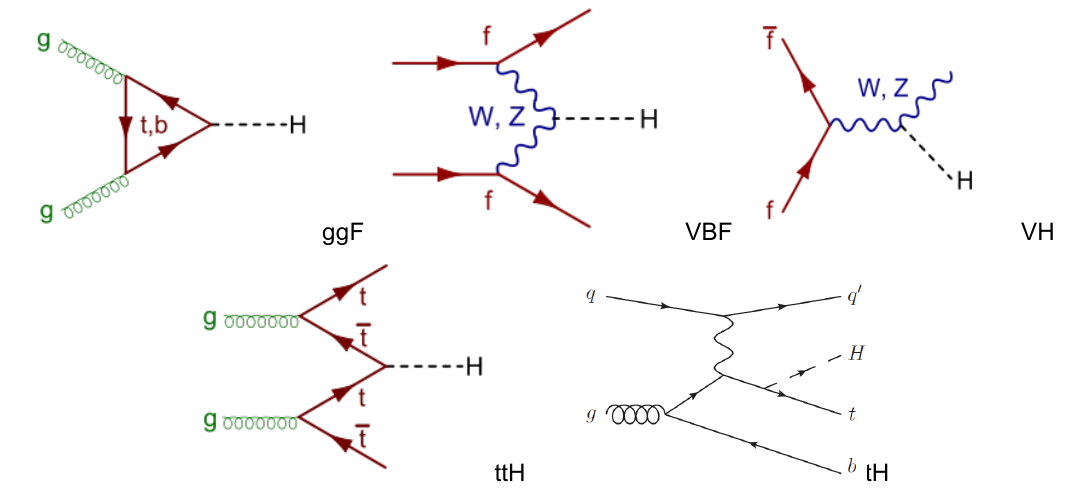
\includegraphics[scale=0.5]{Chapter1/pg.png}
\caption[Higgs production mechanism]{Different Higgs production mechanism, from the most likely to least likely \cite{gamma}\cite{timo}}
\label{psu}
\end{figure}

%\begin{figure}[ht]
%\centering
%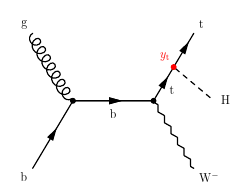
\includegraphics[scale=0.7]{Chapter1/thw.png}
%\caption[$tHW$ mechanism]{$tHW$ mechanism\cite{th1}}
%\label{thw}
%\end{figure}

In the tH process, a Higgs boson is radiated from a single top quark as shown in Figure \ref{psu}. The $tH$ process has gained interest recently\cite{th1}, given that there are few experiments and its production rate (probability) is small, so the detection of Higgs bosons in this channel opens the path to new discoveries.

In particle physics, cross section ($\sigma$) describes the likelihood of two particles interacting under certain conditions.
 Cross sections are expressed in barns, where 1 barn=$10^{-34}$ cm$^{2}$.
The cross section is important in the evaluation of events for specific processes. In order to get the number of events for a specific process, the reaction rate $N$ is determined by the total cross section $\sigma$ and the luminosity L\footnote{The unit of measurement of instantaneous luminosity is cm$^{-2}$s$^{-1}$. }.
%L is called luminosity, that is the number of particle interactions can be produced in a detector per second. 

Therefore, the reaction rate is 
\begin{align} \label{nr}
N_R=\sigma \text{L}
\end{align}
In practice, the luminosity is measured by counting the number of events for a well known process.
\begin{figure}[ht]
	\centering%
	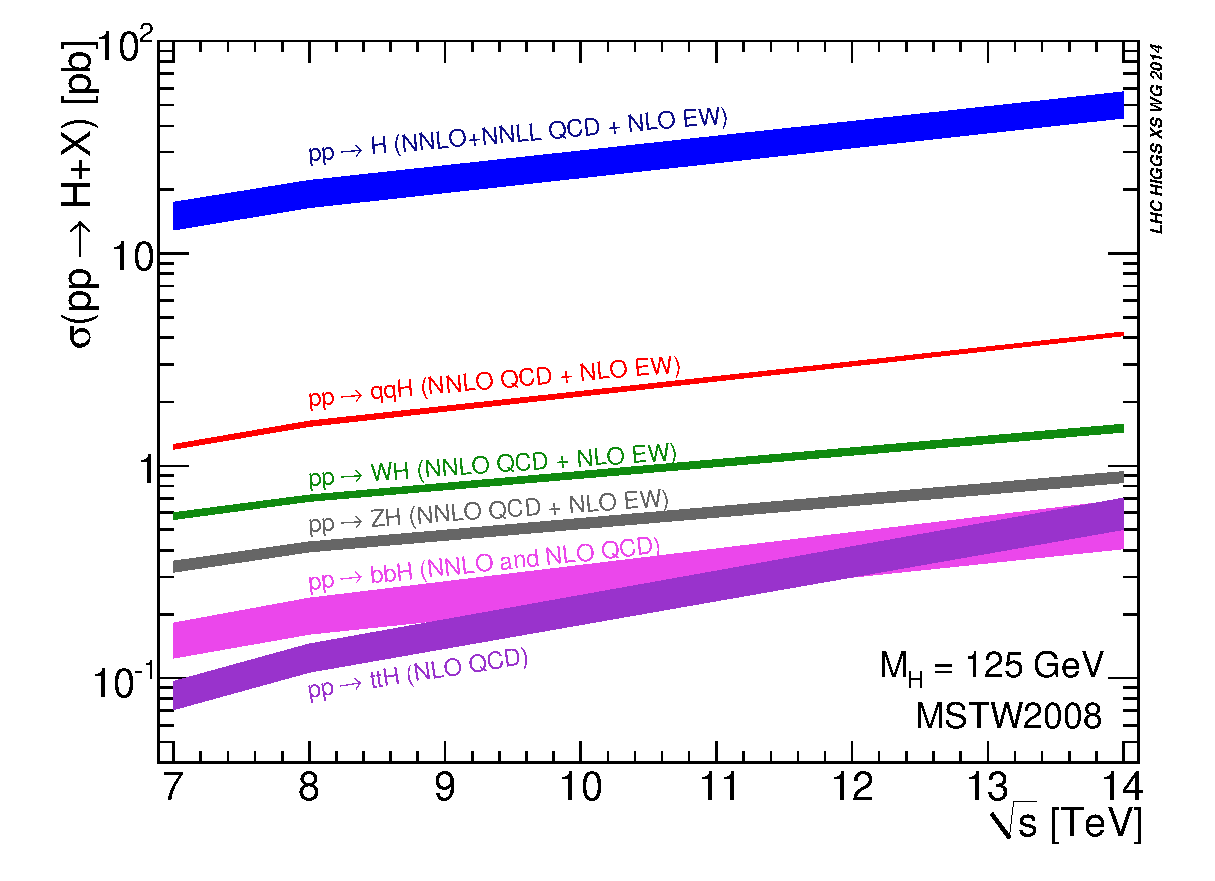
\includegraphics[width=12cm,height=7cm]{Chapter1/7-14xsec.eps}
	\caption[Cross section for different processes generated in a pp collision]{
		Cross section for different processes generated in a pp collision  \cite{dcrosse}}
	\label{csp}
\end{figure}

\begin{table}[ht]
\centering
\caption[Higgs boson production cross sections in pp collisions number of events for  35.9 fb$^{-1}$ ]{	Higgs boson production cross sections in pp collisions for $\sqrt{s}=13$TeV (in pico barn) and number of events for an integrated luminosity of 35.9 fb$^{-1}$ for Run 2  \cite{pd}}
\begin{tabular}{|c|c|c|}
\hline
Production mechanism &
$\sigma$ (picobarns pb) & Number of events \\
\hline
$gg$F & 48.93 & 1756587\\
\hline
VBF & 3.78 & 135702\\
\hline
$WH$ & 1.35 & 48465\\
\hline
$ZH$ &0.88 & 31592\\
\hline
$t\bar{t}$H & 0.50 & 18255\\
\hline
$tH$	& 0.015 & 560.39\\
\hline
\end{tabular}
\label{crt}
\end{table}

 Table \ref{crt} shows the Higgs production cross section for pp collisions and the number of events produced using a integrated luminosity of $35.9 fb^{-1}$, that is the luminosity measured for the Run 2 from LHC on 2016\cite{pd}. Figure \ref{csp} shows the cross sections for each Higgs mechanism process  that comes from pp collisions in relation to colliding energy.
Here we can see that the ggF process has the biggest cross section of all Higgs mechanism and generates the greatest number of events possibles. For the processes tH and $t\bar{t}$H, they have the smallest cross section, so the probability for the processes is low and generates a small number of events. 
\pagebreak

\section{Higgs decay rates}
In particle physics, two important properties are the lifetime and the decay rates of a particle. The lifetime is related to the total decay rate $\Gamma$, that is the probability per unit of time a particle will decay, 
\begin{align}
  dN=-\Gamma N dt
\end{align}
with N the original number of particles before the decay. From here is evident that number of particles left in a decay is 
\begin{align}
N(t)=N_0 e^{-\Gamma t}
\end{align}

%For a particle that decays into several particle, $\Gamma$ is given by
%\begin{align}\label{dm}
%\Gamma=\frac{S}{2\hbar m_n}\int \left| M \right|^2 (2\pi)^4 \delta^4(p_1-p_2-...p_n)\times \prod_{j=2}^n 2\pi \delta (p_j^2-m_j^2 c^2)\theta (p_j^0)\frac{d^4 p_j}{(2\pi)^4}
%\end{align}
%where $m_n$ and $p_n$ are the mass and momentum of the particle n with n=1,2,3,.... S is a statistical factor that avoid identical particles counting. If there are no identical particles, S=1,and for identical particles $S=\frac{1}{s!}$ with s is the number of identical particles. $\mathcal{M}$ is the amplitude which is a momenta function that is calculated acording to the Feynman diagrams.$\theta(p_j^0)$ is a Heaviside function,
%$p_j$ is the outgoing momentum and $p^0_j=E_j/c>0$.\cite{griff}

The number of particles decreases over time exponentially and this can be measured. With this, it is possible determine the mean lifetime\cite{griff}
\begin{align}
\tau=\frac{1}{\Gamma}
\end{align}
In case of the decay rate to a specific process, it is necessary to get the branching fraction of the process. 
The branching ratio for a decay process is the ratio of the number of particles which decay via a specific decay mode with respect to the total number of particles which decay via all decay modes.
\begin{align}
BR_i =\frac{\Gamma_i}{\sum_{i}\Gamma_i}
\end{align}
Where $\Gamma=\sum_i\Gamma_i$ is the total decay width (sum of all partial widths) of the particle.
%Since the dimension of $\Gamma$ is the inverse of time, in our system of natural units, it is measured in inverse seconds, it has the same dimension as mass (or energy)\footnote{Cleaves H.J. (2011) Branching Ratio. In: Gargaud M. et al. (eds) Encyclopedia of Astrobiology. Springer, Berlin, Heidelberg}. 
The lifetime of the Higgs boson is predicted to be 1.56 $\times$ $10^{-22}$ seconds and corresponds to $\Gamma_H$ of about 4 MeV, but has not yet been measured due to the detector resolution\cite{cms-manual}.

\begin{table}[ht] 
\caption[SM Higgs boson branching ratios for $M_H$ =125 GeV]{SM Higgs boson branching ratios for $M_H$ =125 GeV \protect \cite{pd}}
\centering
\begin{tabular}{|c|c|}
\hline
Higgs decay & Branching ratio (BR)\\
\hline
$H \rightarrow$ b$\bar{b}$ &$58.4\%$ \\
\hline
 $H \rightarrow$ $W^+W^-$ &$21.4\%$ \\
\hline
$H \rightarrow$ $\tau^+ \tau^-$ & $6.27\%$\\
\hline
$H \rightarrow$ ZZ &$2.62\%$\\
\hline
$H \rightarrow$ $\gamma\gamma$ &$0.227\%$\\
\hline
$H \rightarrow$ Z$\gamma$ &$0.153\%$\\
\hline
$H \rightarrow$ $\mu^+\mu^-$ &$0.0218\%$\\
\hline
\end{tabular}
\label{higgs1}
\end{table}
The decay $H \rightarrow$ $b\bar{b}$ has a branching ratio a bit more than 50$\%$. The decay $H \rightarrow$ $\mu^+\mu^-$ has a very low branching ratio. This decay is very rare but not impossible to detect in the future. %In this work the majority of the Higgs decays detected are from $WW$, $ZZ$, $\tau \tau$.

\section{$tH$ production mechanism}
The production of $tH$, where a Higgs boson can be radiated
either from the top quark or from the exchanged $W$ boson in the two dominant leading order
diagrams shown in Figure \ref{newth} provides a unique opportunity to study the relative sign of the Higgs top coupling.
In practice, we do not directly measure the Yukawa couplings. Instead, modifier parameters $k_t$ and $k_V$ are introduced in the analysis to represent deviations from the Yukawa coupling values. 
In the SM, the two diagrams interfere negatively and thereby suppress the production cross section.
Any deviation from the SM coupling parameters can lead to a large enhancement of the event rate. 
In this project we consider a modified model with $k_t$=-1, which leads to a constructive interference and a $tH$ cross section more than ten times. 
 %$\kappa_t$ and $\kappa_V$ are the modifier of the coupling parameters discussed in section 1.5, where $\kappa_t$ is for the top and $\kappa_V$ for $W$ boson. 

\begin{figure}[ht]
	\centering
	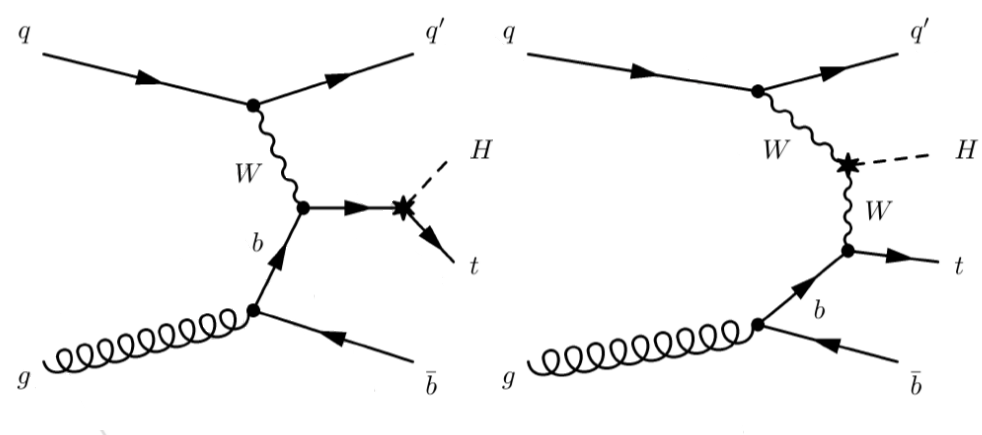
\includegraphics[scale=0.5]{Chapter1/newtHq.png}
	\caption[$tH$ mechanism]{$tH$ mechanism. Higgs radiated from a top quark (left). Higgs radiated from a W boson (right) \protect \cite{bb}} \label{newth}
\end{figure}
\pagebreak
\end{chapter}














	%!TEX root = ../thesis.tex
%*******************************************************************************
%****************************** Second Chapter *********************************
%*******************************************************************************

\chapter{The LHC and CMS}

\section{The Large Hadron Collider}

The Large Hadron Collider (LHC) is one the  largest and most powerful particle accelerator in the world. It came on operation on 10 September 2008 and it is the most recent addition from the  European Organization for Nuclear Research (CERN).  The LHC is a 27 kilometer ring composed of  superconducting magnets with accelerating structures to boost the energy of the particles. \\

The LHC is designed to accelerate particles to high energies and generate collisions. There are several
experiments installed along the LHC ring. One of them is ATLAS, located on Point 1 between the two injection lines, which is a general purpose detector. At point 5 is another general purpose detector: the compact muon solenoid  (CMS). A particle detector optimized for heavy ion physics, ALICE, is located at Point 2 and LHCb, a detector designed for B physics, is located at Point 7\cite{cern1,cern2}.
\\

Inside the accelerator, two high energy particles beams travel at
close to the speed of light before they collide. 
In order to make them collide, beams travel in opposite directions in separate beam pipes, 
two tubes kept at ultrahigh vacuum. 
By using of superconducting electromagnets that generates a powerful magnetic field, the beams are guided around the accelerator ring. 
The electromagnets are built from coils of special electric cable that operates in a superconducting state, efficiently conducting electricity without resistance or loss of energy. For that, it is required to have  magnets to a temperature of  $‑271.3$ C. 
To reach such temperatures, a system of liquid helium is connected to the accelerator\cite{cern2}.

\pagebreak

\begin{figure}[!htbp]
\centering
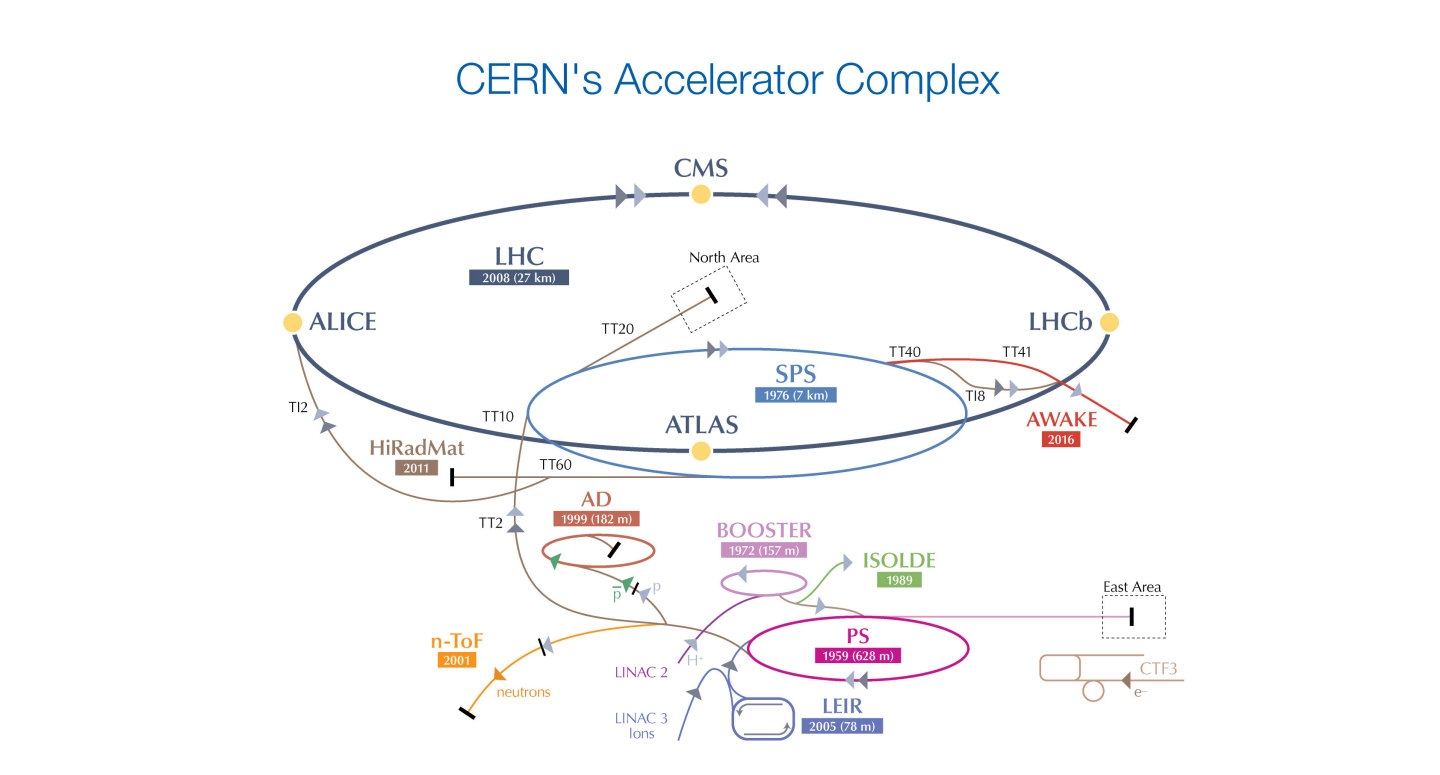
\includegraphics[width=17cm,height=11cm]{Chapter1/cern.jpg}
\caption[Large hadron collider from CERN]{Large hadron collider from CERN\cite{cern1}} \label{lhc}
\end{figure}


Protons in the LHC start out as hydrogen atoms stripped of their electrons. The first accelerating stage the protons are subjected to is a linear accelerator, Linac2,
which accelerates them up to 50 MeV. The protons are then sent into the
Proton Synchotron Booster which accelerates them up to 1.4 GeV before sending them to the Proton Synchotron (PS). The protons leave the PS at 25 GeV before entering the Super Proton Synchotron (SPS), which accelerates them to the LHC injection energy of 450 GeV. After this stage, the beam is ready to be injected into
the LHC through one of two injection lines with 6.5 TeV\cite{cern3}.


\begin{table}[!htbp]
\centering
	\caption[Accelerator operation energies]{Accelerator operation energies\cite{cern1,cern3}}
	\begin{tabular}{|c|c|}
		\hline
		Accelerator & Energy \\
		\hline
		Linac 2 &  50 MeV \\
		\hline
		PS Booster & 1.4 GeV \\
		\hline
		Proton Scyncroton (PS) & 25 GeV\\
		\hline
		SPS &  450 GeV\\
		\hline
		LHC & 6.5 TeV\\
		\hline
	\end{tabular}
\end{table}
\pagebreak
Inside the detectors, collided protons generates an amount of particles such as pion and kaons, which are the most commons, created by the jet particles that were created after the collision. Besides of the particles created by the quarks of the proton, gluons are also radiated and create new particles and photons are radiated too. \\
During the collision time, the main  detectors of LHC capture the energy 
and save the data in supercomputers. Those high end computers starts to measure the signals in order to assign a type of events.
\\

The main objective of the LHC is to study the nature of electroweak symmetry breaking for the Higgs mechanism of the SM. 
Alternatives to the Standard Model that involves different symmetries are also put on test. With the exploration of theses theories, people hope for a discovery that guide them toward a unified theory, so the importance to accelerate particles to higher energy scales.
\\
The LHC has a schedule where there is a period of experiments that last for three or four years. Ending the experimental time, the engineers of the LHC start the maintenance.

\begin{figure}[!htbp]
\centering
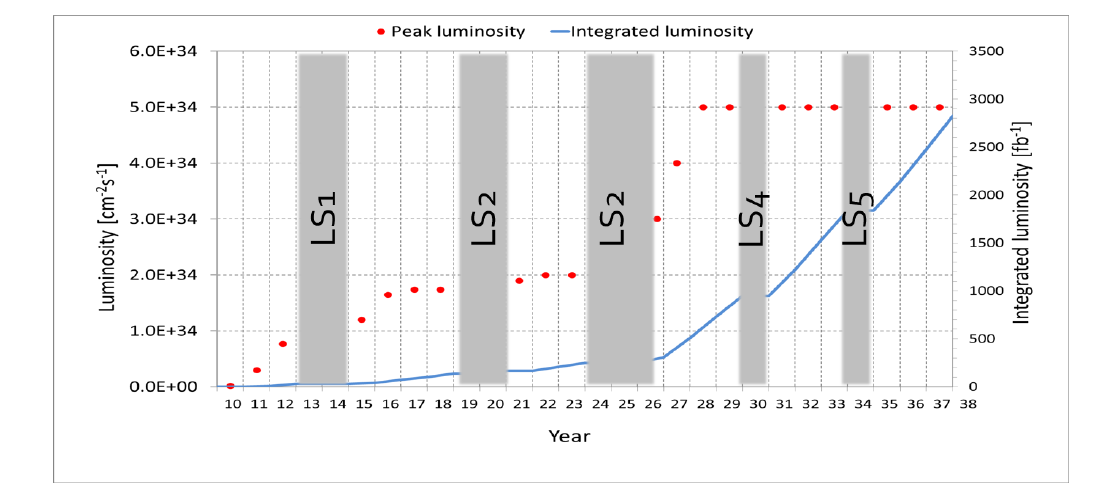
\includegraphics[scale=0.5]{Chapter2/lum6.png}
\caption[LHC schedule, including future plans for increase the center of mass energy and luminosity. The periods labeled LS are the maintenance periods]{LHC schedule, including future plans for increase the center of mass energy and luminosity. The periods labeled LS are the maintenance periods\cite{cern3}.}
\label{lhc-lumi}
\end{figure}
From the figure \ref{lhc-lumi}, shows the Large Hadron Collider forecast for the increase of luminosity for the next years. Red dots are peak luminosity expected to reach and blue line is integrated luminosity. In the year 2018, the maximum integrated luminosity is around 150 $fb^{-1}$\cite{cern3}. From 2019 to 2021 the second phase of maintenance, where engineers increase the performance of the accelerator, give maintenance to the system and introduce new components to the complex. After that period, the LHC starts new collision period at even higher energies in order to explore new particle phenomena.

\pagebreak

\section{The Compact Muon Solenoid}	
The Compact Muon Solenoid (CMS) is a detector with multiple uses in the LHC and part of the main experiments at CERN. Located underground in the France- Switzerland border, in the city of Cessy, France.
This detector was designed in the early 1990s, based on the mass limit of the Higgs boson,  and put on operation in 2008,  it has a big solenoid that generates a great magnetic field of 4 teslas with the objective to separate particles after a particle collision.
 The detector is 21 metres long, 15 meters wide, 15 meters high, it has a diameter of 5.9 m with a weight of 12000 ton. The reason for such a strong magnetic field is to obtain a better momentum resolution.
 The magnetic flux is returned via a 1.5 m thick  iron yoke instrumented with four stations of muon
 chambers.



\begin{figure}[!htbp]
	\centering
	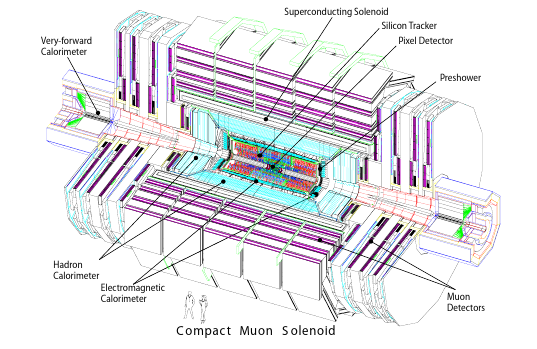
\includegraphics[width=10cm,height=6cm]{Chapter2/cms2.png}
	\caption[View of Compact muon solenoid (CMS)]{View of Compact muon solenoid (CMS)\cite{cms-manual}}\label{cms}
\end{figure}
There are many layers of detectors to register different kinds of energy signals. But since muons go through materials very easy, the complex is buried 100 meters underground.\\ 

The CMS experiment is composed of several detector layers  that allow identify and save different types of energy signals  and it is saved in a powerful supercomputers that separate and classify the data according to certain variables. The general parts of the CMS are the Silicon Tracker, an Electromagnetic Calorimeter,a Hadron Calorimeter, the solenoid (superconducting magnet) and the Muon Detector. \\

\begin{table}[ht]
	\caption[Characteristic of the CMS superconducting solenoid]{Characteristic of the CMS superconducting solenoid\cite{cms-manual}}
	\centering
	\begin{tabular}{|c|c|}
		\hline
		Field strength & 4 T \\
		Inner Bore & 5.9 m \\
		Length & 12.9 m\\
		Number of Turns & 2168\\
		Current & 19.5 kA\\
		Stored energy & 2.7 GJ\\
		\hline
	\end{tabular}
	\label{tab:my_label}
\end{table}



%The trigger or event selection process must reduce the approximately 1 billion interactions per second to more less than 100 events per second for storage and subsequent analysis.\\

 The objectives of the CMS experiment are numerous. One of them is
identification of muons by measuring the momenta and scattering angle. Muons can be produced in interesting events like Higgs, $W^{\pm}$ and $Z$ boson decays.%Search for evidence  and give proof of super symmetry  for show evidence of BSM (Beyond Standard Model). Detection of massive vector bosons $W^\pm$ and Z via $e^+e^-$ and $\mu^+ \mu^-$ decays.\\
%Search for extra dimensions from BSM theory that could be related to production of particles and quantum gravity. Study of QCD, electroweak and flavor physics to detect new decays predicted by SM at higher energies. Heavy ions collision experiments for the study of production of  very strongly interacting nuclear matter\cite{cms-manual}.
This experiment along the ATLAS experiment discovered the Higgs boson in 2012.
\\


\subsection{Silicon Tracker}
The Silicon Tracker is the first of the main subdetectors of CMS from inside to outside. The Tracker is composed of two sub components: Pixel and  Strip detectors. The outer radius of the  tracker is 110 cm, and its total length is 540 cm. The tracker coverage is $|\eta|<2.4$\footnote{$\eta$, called pseudorapidity, is a coordinate where $\eta=-\ln{\tan{\frac{\theta}{2}}}$}.\\

In the Pixel barrel section, there are 3 layers of pixel sensors with radii of 4.4, 7.3 and 10.2 cm with a length of 53 cm. Each pixel has an area of 100 $\times$ 150 $\mu m^2$.  The barrel section has 768 pixel modules.
%The barrel section of the silicon tracker is divided in inner and outer barrel, where the inner section is shorter than outer barrel along with 3 inner disk between the transition region between barrel and endcap sections because avoids shallow track crossing angles.  
The Pixel endcap has 2 disks on each side placed at 34.6 and 46.5 cm in the z axis. Each disk covers radii from 6 to 15 cm and is divided into 24 blades with 7 modules each blade.
They are assembled in a turbine-like geometry that contains a total of 672 pixel modules. %with 7
%different modules in each blade.
\\

 %The outer radius of the  tracker is 110 cm, and its total length is 540 cm. \\
 %Here, silicon microstrip detectors are placed in the r axis (cylindrical coordinates),  between 20 and 110 cm.
%In the endcap section 2 pixel and microstrip layers are placed in each endcap. The endcap have 2 disks of radii from 6 to 15 cm placed at 34.6 and 46.5 cm in the z axis. The endcap disks comprise 672 pixel modules with 7
%different modules in each blade.
The Strip Detector is divided in 4 sections: Tracker inner barrel (TIB), tracker outer barrel (TOB), tracker encap (TEC) and tracker inner disk (TID). The region that cover the barrel section is $|z|<65$ cm for TIB and $|z|<110$cm for TOB. The first two are composed  of silicon sensors layers of 4 and 6 layers respectively.  The TEC has 9 disk extending in the region 120 cm > $|z|$ > 280 cm. The 
TID comprises 3 small disks that fill the gap between the TIB and the TEC.


The Strip Detector have almost 15 400 modules, mounted on
carbon-fiber structures and housed inside by a temperature controlled outer support tube. The operating temperature must be around -$\ang{20}$C. 
The total area of the pixel detector is around 1 $m^2$ and the silicon strips is 200 m$^2$. 
The inner tracker comprises 66 million pixels and 9.6
million silicon strips \cite{cms-manual}.
A full coverage of the Tracker is shown in figure \ref{pixel2}
\\

\begin{figure}[ht]
	\centering
	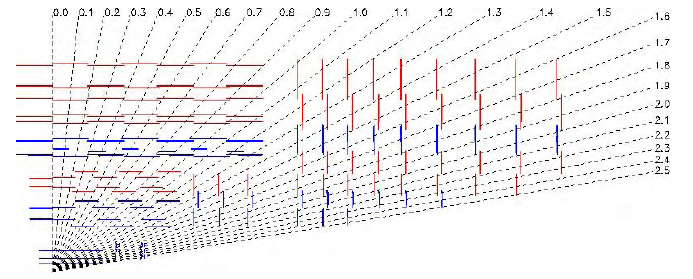
\includegraphics[scale=0.7]{Chapter2/pixel2.png}
	\caption[The Tracker layout distributed in terms of $\eta$]{The Tracker layout distributed in terms of $\eta$\cite{cms-manual}.}
	\label{pixel2}
\end{figure}
During the particle collision, it generates a lot of different particles that pass first through the inner tracker, interacting with the sensors layers and registering the particle path.
By reconstructing the path of the particles, it is possible to generate a track, which allows to measure the momentum of the particle by calculating its curvature. The tracker is used to reconstruct the path of charged particles (e.g. electrons, muons, pions). The most important objects of study are the momentum and the vertex (origin of the track). The efficiency of the tracker is estimated by using samples of muons and pions with $p_t$ of 1,10 and 100 GeV. 
For muons the efficiency of the tracker is shown in \ref{efi}
\begin{figure}[!htbp]
	\centering
	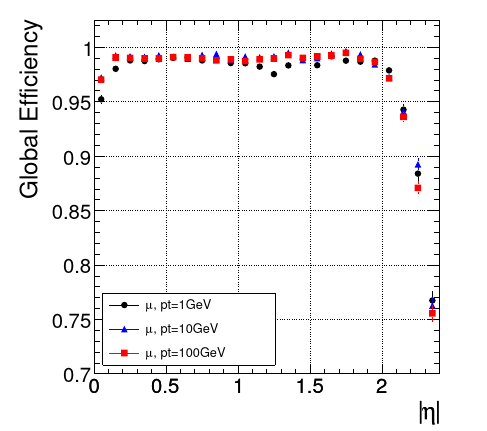
\includegraphics[width=10cm,height=6cm]{Chapter2/tracker.png}
	\caption[Total reconstruction efficiency for muons]{Total reconstruction efficiency for muons\cite{cms-manual} }\label{efi}
\end{figure}
\\
According to figure \ref{efi}, the efficiency of the tracker is around 98 $\%$ for $|\eta|<2$. The resolution of the tracker  for muons with $p_t$=100 GeV is around 1-2 $\%$.\\
Of course, this is a first stage of the measurement of particle momentum because the other detectors are used to increase and improve the measurement and reconstruction of the particle path.

\subsection{Electromagnetic calorimeter}

The electromagnetic calorimeter or ECAL is a calorimeter composed of 61200 lead tungstate (PbWO$_4$) crystals that act as scintillating crystals (emits light when particles interact with the crystal). These calorimeters are mounted in the central barrel and closed by 7324 crystals in the both endcaps. The barrel section  of the ECAL covers the range $|\eta| < 1.479$. The crystals in the barrel have a pyramid shape and their cross section is 22$\times$22 mm$^2$ at the front face and 26$\times$26 mm$^2$ at rear face. The crystal length is 230 mm. The EB (barrel section of ECAL) has a inner radius of 129 cm\cite{cms-manual}\\

The endcaps cover have the  range 1.479 < $|\eta|$ < 3.0. The distance between the interaction point and the endcap is 3.144 m. The endcap has  identically shaped crystals grouped in
mechanical units of 5×5 crystals. The crystal cross section for the rear face is 30 $\times$ 30 mm$^2$, and for front face cross section is 28.62 $\times$ 28.62 mm$^2$ with length of 220 mm.
\\
\begin{figure}[!htbp]
	\centering
	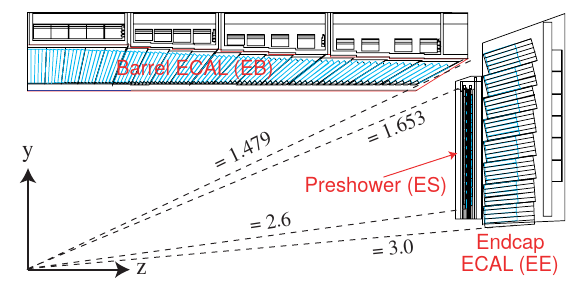
\includegraphics[width=10cm,height=6cm]{Chapter2/ecal.png}
	\caption[View of the ECAL]{View of the ECAL\cite{cms-manual}}\label{ecal}
\end{figure}
In the barrel, there photo detectors called avalanche photo diodes (APD), made of silicon with a active area of  5 $\times$ 5 mm$^2$ with 2 glued to the back of each crystal.  At the endcap, the photo detectors are vacuum photo diodes (VPT), made of with an anode of copper mesh (10 $\mu m$), allowing to operate in the magnetic field. VPT have a size of 25 mm in diameter, glued to the back of each crystal.\\


There is also a preshower detector, which principal function  is to identify neutral pions in the
endcaps within the region 1.653 < |$\eta$| < 2.6. It also helps the identification of electrons
against minimum ionizing particles, and improves the position determination of electrons and photons.
\\

As its name says, the ECAL is mainly used for the electron detection, but also detects, photons, and neutral pions. The charged particles reach the crystals that provokes the photo diodes detect energy.\\
The  resolution of the ECAL is estimated by using a test beam and registering the energy signals. The resolution for electrons with energies of 120 GeV, it has obtained a resolution of 0.5$\%$.
 
 %that a electron is separated, and regrouping in other place due to the electric field generated  by the voltage source. 
 %The ES is a sampling calorimeter with 2 layers: lead
%radiators initiate electromagnetic showers from incoming photons/electrons whilst silicon
%strip sensors placed after each radiator measure the energy deposited and the transverse shower profiles.


\subsection{Hadron calorimeter}
The hadron calorimeter (HCAL) along the ECAL, form a complete calorimeter that allows to measure the jets and missing transverse energy. HCAL is located in the barrel and the endcaps, surrounding the ECAL and affected by the magnetic field generated by the solenoid. The Barrel section (HB) and endcap section (HE)  cover the pseudorapidity 0 < $|\eta|$ < 1.3 and  1.3 < $|\eta|$ < 3.0 respectively.\\ 


The HB is an assembly of two half barrels, composed of 18 wedges. Each wedge has 17 active layers composed of scintillator tiles with 16 layers of 
absorbent metal (brass and stainless steel). Each tile has a size of $\Delta \eta × \Delta \phi$ = 0.087 $\times$ 0.087. Light of scintillator is collected by a single wave
length shifting fiber (WLS) for each scintillator tile. The wedge has a inner radius of 1777 mm to an outer radius of 2876.5 mm. 
\\

HE is composed by brass absorbent plates, with the thickness of 78 mm, and a total of  19 scintillator layers with a thickness of 3.7 mm.  HE is sectioned in 5 in $\phi$ to match the barrel wedges. %HO scintillators follow the HCAL barrel tower geometry in $\eta$ and angle $\phi$, that is , the geometry of the barrel muon system. Divided by 5 rings of 2.54 wide, composed of the scintillators on either side of the tail catcher iron of 18cm thick at radial distances of 3850 and 4097 mm respectively. \cite{cms-manual} 
\\
\begin{figure}[!htbp]
	\centering
	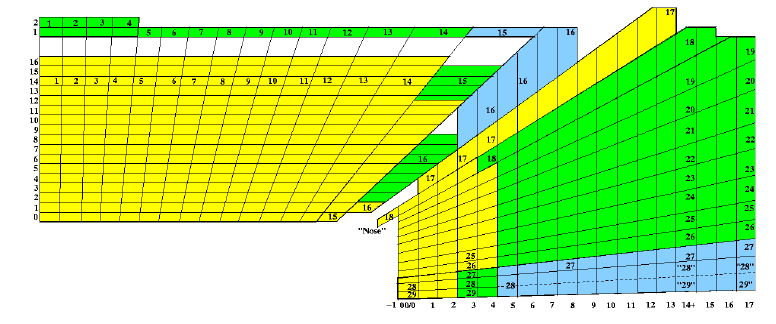
\includegraphics[width=10cm,height=6cm]{Chapter2/hcal.png}
	\caption[View of the CMS HCAL showing the different layers and tower regions. In the endcap, the towers are defined with two longitudinal segments as shown by the colors]{View of the CMS HCAL showing the different layers and tower regions. In the endcap, the towers are defined with two longitudinal segments as shown by the colors\cite{cms-manual}}\label{hcal}
\end{figure}
The outer barrel hadron calorimeter (HO) consists of layers of scintillator with  thickness of 10 mm, located outside of the
magnet coil that cover the region -1.26 < $|\eta|$ < 1.26.\\
There is also a forward calorimeter (HF) located at 11.2 m from the interaction point, that cover the region of 2.9 < $|\eta|$ < 5. They are made of
steel absorbent and embedded radiation hard quartz fibers,which collects 
Cherenkov light\cite{cms-manual}.% that is  when a charged particle travels through matter faster than light can, resulting in a blue light emmision of the material. 
%The length of the fibers are 1.65 m and 1.43 m, which are alterned with a 5 mm of separation. 
\\
  
The tiles are arranged in a tower pattern in the  $\eta-\phi$ space, projected to the interaction point.  In total there
are 4176 towers. The towers are used as input to several jet reconstruction algorithms.

The HCAL measures the energy of hadrons,such as the pions and kaons. 
The energy resolution of the HCAL was estimated using a test beam of pions. For 100 GeV pions, the resolution obtained is 12$\%$.
 %By using the info given by the HCAL, it is possible reconstruct the track in order to calculate the momentum of the particles. 

\subsection{Muon Detector}
%The muon detector system  %has 3 primary functions: muon
%triggering, identification, and momentum measurement\cite{cms7}. 
%The process utilized in the CMS muon chamber systems is gas ionization. Those gas-ionization particle detectors are arranged in a cylindrical barrel region and planar endcaps, in order to meet the geometry of the solenoid.The barrel detector is built with 4 layers of 250 chambers inside the magnet return yoke.\cite{cms-manual}
The Muon Detector has three main subdetectors: the drift tubes chambers (DT), the cathode strips chambers (CSC) and the resistive plate chamber (RPC). 
The  DT's, CSC's and RPC's are shown in the figure \ref{dt}.
 \\
 
The DT chambers cover the barrel section $|\eta|<1.2$, composed of rectangular gas filled active cells. Those cells have a transverse size of 42 $\times$ 13 mm$^2$ with a 50 $\mu m$ diameter anode wire at the center that operates at voltages of over 3600 V. The gas used in this cells is a mix of Ar and CO$_2$ with a proportion of 85 $\%$ and 15 $\%$. There are 250 chambers in 4 layers inside the magnet return yoke, with radii of approximately 4.0, 4.9, 5.9 and 7.0 m from the beam axis  and 12 sections covering  30$^\circ$ in $\phi$ each one.
\\
\begin{figure}[!htbp]
	\centering
	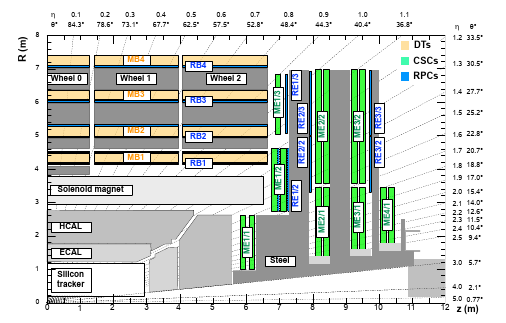
\includegraphics[width=11cm,height=7cm]{Chapter2/csc}
	\caption[Cross section of a quadrant of the CMS with axis parallel to the beam (z axis) horizontally and the radius of the detector in terms of the $\eta$]{Cross section of a quadrant of the CMS with axis parallel to the beam (z axis) horizontally and the radius of the detector in terms of the $\eta$\cite{cms-manual}.}
	\label{dt}
\end{figure}

The CSC's are located in the endcap regions 0.9 < $|\eta|$ < 2.4. The CSC's are installed on the face of steel disks perpendicular to the beam. 
Each CSC has a trapezoidal shape and consist of 6 gas gaps between 7 metal plates, where each gap contains  copper cathode strips and anode wires running almost perpendicularly to
the strips, with a diameter of 50 $\mu m$ separated by 3.16 mm.  
%CSC is composed of 6 layers that measures the $\mu$ position in the r-$\phi$ coordinate plane. 
The chambers use a gas mixture of 50$\%$ CO$_2$, 40 $\%$ Ar and 10$\%$ CF$_4$. The muon endcap system comprises 468 CSCs in the 2 endcaps \cite{cms-manual,cms7}.
%Together with DT, cover the $|\eta|< 2.4$. These systems can each identify the collision crossing that generated the muon and trigger on (recolect) the transverse momentum ($p_T$). 
\\

The RPC are located in the barrel and endcap regions that covers the range o $|\eta|<1.6$. The main purpose is to trigger events with muons. 
RPC's are structured with a double gas filled gap and readout strips between the gaps.\\
 The gas mix used in the RPC consist of 95.2$\%$ Freon
($C_2 H_2 F_4$ ), 4.5$\%$ isobutane ($C_4 H_{10}$), and 0.3$\%$ sulphur hexafluoride (SF$_6$ )\cite{cms7}.\\


 %The vertical lines represent the endcap and the horizontal the muon barrel. The orange sections are the DTs , where the 4 DTs are labeled MB,CSC marked in green are labeled ME or muon endcap and RPC are the blue lines that are located in the barrel and the endcap. RPC are labeled RB and RE respectively. 

%The produced muons are measured in three zones: in the inner tracker, after the coil, and in
%the return flux. Measurement the momentum of muons in the muon detector is determined by the muon bending angle at the exit of the 4T coil with the interaction point as the origin of the muon\cite{cms7}\cite{cms-manual}.
%The resolution of the muom detector is based on simulations taking account with the geometry and a test beam. 
The main purpose of the Muon System Detector is to identify muon tracks. 
The efficiency of the muon system is estimated by using single muon samples simulated with $p_t$=10, 50, 100, 500 and 1000 GeV. The results are shown in the figure \ref{mu-efi}.
\begin{figure}
	\centering
	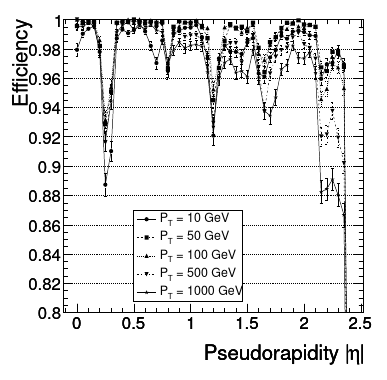
\includegraphics[width=0.4\linewidth]{Chapter2/mu-efi}
	\caption[Muon reconstruction efficiency in terms of $\eta$ and $p_t$]{Muon reconstruction efficiency in terms of $\eta$ and $p_t$\cite{cms-manual}}
	\label{mu-efi}
\end{figure}
The graph shows an efficiency of approximately 98$\%$ in the the fully instrumented regions. In the intersection regions, there are drops in efficiency  due to the separation of the chambers. % There is a reduction of the efficiency to 6$\%$, which corresponds to the $\eta$  position for the separation.

	%!TEX root = ../thesis.tex
%*******************************************************************************
%****************************** Third Chapter **********************************
%*******************************************************************************
\chapter{Event reconstruction and selection}
During the proton collision, many types of processes happen whose information are saved in the CMS data storage system. But the events are only saved if they fulfill certain conditions compatible with the signal. 
For the tH process , the search is based on the presence of  a pair of muons with the same sign. The rest of the processes that also generates a pair of muons with the same sign will be considered backgrounds.  
\section{Signal Event Topology} 
In this search, top quark decays to $Wb$ and from the $W$ boson decays to a muon and a neutrino. The Higgs decays to a pair of opposite sign $W$ bosons, where one of the bosons can decay to a $\mu$ and its neutrino. This is the main process that generates events with two same sign muons.The tH process topology is shown in the figure \ref{jet}.\\

Figure \ref{jet}, also shows a b-jet that comes from the tH process.  Finally there is a forward  quark jet (highest $\eta$ value) generated from the initial collision. Additional jets or leptons can be generated from the other $W$ boson.
\\
	
  %The W bosons can also decay to quarks that generate jets. 
Due to the small cross section of the $tH$ process, the amount of $tH$ events is low compared to other Higgs production processes. 
Table \ref{tdecay} shows several processes that generate same sign muon events for $t$H. These numbers do not consider the detection efficiency.
  %But also tH process can generate the final states from $\tau$ decays but with a low probability. Some of them have probability near zero , but not impossible . %In graphics, these low probability processes would be very small figures that barely manifest.

%For the tH process, the largest contribution comes from Higgs decays to WW (about 75$\%$), followed
 %y $\tau \tau$ (about 20$\%$) and ZZ (about 5$\%$).

	\begin{figure}[!htbp]
		\centering
		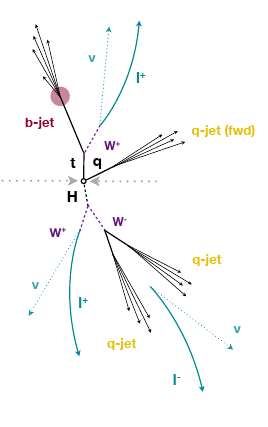
\includegraphics[scale=0.9]{Chapter1/jet.png}
		\caption{Topology of $t$H process which generates two same sign muons , a forward jet and a b-jet.} 
		\label{jet}
	\end{figure}
%Quarks and gluons only exist in bound states. Because of it, we cannot isolate quarks except the top quark because of their decay times that don't form a bound state. When two quarks are separated, the strong force interacting between them increases. The energy transforms into quark anti-quark pairs. The hadronization results in a jet of particles. 

\pagebreak


\section{Backgrounds}
Several processes contribute to the background in this search:
\begin{itemize}
		\item $\bm{t\bar{t}W^{\pm}}$ and $\bm{t\bar{t}Z}$ $\bm{(t\bar{t}V)}$: One muons comes from a top and the other comes from the vector boson.
			\item $\bm{W^{+}Z}$: Diboson production with leptonic decays. One muon comes from $W$ boson and the other from $Z$ boson.
		\item $\bm{W^{\pm}W^{\pm}}$:A pair of same sign $W$ bosons generate a muon each one.
		\item $\bm{tZq}$: Processes with single top quarks associated  with a Z boson, where $Z\rightarrow \mu^+ \mu^-$, also contribute to the background.
	\item $\bm{t\bar{t}t\bar{t}}$:In these type of events, one $t$ decays to $Wb$ and $W$ decays to a muon. The second muon comes from the other top decay.
	%Backgrounds are estimated directly from simulated events$\%$ which are corrected for data/MC differences and $\%$ inefficiencies in the same way as signal events. 
		\item$\bm{W^{+}W^{-}Z}$, $\bm{ZZZ}$ and $\bm{W^{+}ZZ}$ ($\bm{VVV}$): The leptonic decays of the $W$ or $Z$ bosons generate at least two same sign muons.
	\item $\bm{tZW^{+}}$:One muon comes from the $Z$ while the other same sign muon can come from $t$ or $W$. 
	\item $\bm{ZZ}$: Each muon comes from $Z$ boson decays.
			\item $\bm{t\bar{t}H}$: This Higgs  production mechanism is considered a background in this analysis. The muons in this cases comes from one top and Higgs decays. 
	\item $\bm{Fakes}$:This background refers to events where two muons come from  $b$ meson decays in jets.
\end{itemize}
Table \ref{back} show the decay chains and production cross section for background. Due to small expected event yields, the processes $W^\pm$ $W^\pm$ ,$tZq$,$t\bar{t}t\bar{t}$ $VVV$, $tZW^+$ and $ZZ$   are grouped as one called Rares in the results below.

\pagebreak 

\begin{table}[!ht]
	\caption{Expected number of events for different $tH$ decay chains assuming integrated luminosity of 35.9 fb$^{-1}$. $l$ represents $\mu^{\pm},e^\pm , \tau^\pm$.}
	\begin{tabular}{|l|c|c|}
		\hline
		Decay chain & BR & Events\\
		\hline 
		\small{$tH \rightarrow$ $W^+bW^+ W^-$ $\rightarrow$ $\mu^+$ $\nu_\mu b$ $\mu^+\nu_\mu$  $q \bar{q}'$ } &\small{2.096 $\times$10$^{-3}$} &  1.173  \\
		\hline
		\small{$tH \rightarrow W$$^+ b$$W^+$ $W^-$ $\rightarrow$ $\mu^+\nu_\mu b$ $\mu^+\nu_\mu$ $l^- \bar{\nu_l}$ } &\small{3.37 $\times$ 10$^{-4}$} &0.899 \\
		\hline
		\small{$tH \rightarrow$ $W^+ b$ $\tau^+ \tau^-$ $\rightarrow$ $\mu^+ \nu_\mu b$  $ \mu^+ \nu_\mu \bar{\nu_\tau} l^-\bar{\nu_l} \nu_\tau$} &\small{3.637$\times$10$^{-4}$}&0.203 \\
		\hline
		\small{$tH \rightarrow$ $W^+ b$ $W^+ W^-$ $\rightarrow$ $\tau^+ \bar{\nu_\tau}b$ $\mu^+ \nu_\mu$  $q\bar{q}$ $\rightarrow$ $\mu^+ \nu_\mu$ $\bar{\nu_\tau}$ $\bar{\nu_\tau} b\mu^+ \nu_\mu$  $q \bar{q}$} &\small{1.890$\times$10$^{-4}$}&0.105  \\
		\hline
		\small{$tH \rightarrow W^+ b \tau^+ \tau^-$ $\rightarrow$ $\mu^+$ $\nu_\mu b$ $\nu_\tau$ $\mu^+$ $\nu_\mu \bar{\nu_\tau}$} $q \bar{q}$  &
		\small{1.681 $\times$10$^{-4}$} & 0.094 \\
		\hline
		\small{$tH \rightarrow W^+ b$ $W^+ W^-$ $\rightarrow$ $\tau^+ \bar{\nu_\tau} b \mu^+ \nu_\mu l^- \bar{\nu_l}$ $\rightarrow$ $\mu^+\nu_\mu$ $ \bar{\nu_\tau} \bar{\nu_\tau} b \mu^+ \nu_\mu l^- \bar{\nu_l}$} &\small{3.045$\times$10$^{-5}$}& 0.017\\
		\hline
		\small{$tH \rightarrow W^+ bZZ$ $\rightarrow$ $q \bar{q} bZZ$ $\rightarrow$ $q \bar{q}  b \mu^+ \mu^- \mu^+ \mu^-$} & \small{1.966$\times$10$^{-5}$} &0.011\\
		\hline 
		\small{$tH \rightarrow$ $W^+ b$ $\tau^+ \tau^-$ $\rightarrow$ $\tau^+ \bar{\nu_\tau}b$ $\mu^+ \nu_\mu \bar{\nu_\tau} $  $q\bar{q}' \nu_\tau$ $\rightarrow$  $\mu^+ \nu_\mu \bar{\nu_\tau}\bar{\nu_\tau} b \mu^+ \nu_\mu \bar{\nu_\tau} $  $q\bar{q}' \nu_\tau$ } &\small{1.549 $\times$10$^{-5}$} &  0.008  \\
		\hline
	\end{tabular}
\label{tdecay}
\end{table}



\begin{table}[!ht]
	\caption{Main backgrounds and their same sign $\mu\mu$ decay process }
	\centering
	\begin{tabular}{|c|l|}
		\hline
		Background &  Decay process \\
		\hline
		$t\bar{t}W$  &$t\bar{t}W$  $\rightarrow$  $W^+ b W^- \bar{b}$ $\mu^+\nu_\mu$ $\rightarrow$ $\mu^+ \nu_\mu b$ $\mu^- \bar{\nu_\mu} \bar{b}$ $\mu^+ \nu_\mu$\\
		\hline
		$t\bar{t} Z$ & $t\bar{t} Z$  $\rightarrow$ $W^+ b$  $W^-\bar{b} \mu^+ \mu^-$ $\rightarrow$ $\mu^+ \nu_\mu b$ $\mu^- \bar{\nu_\mu} \bar{b}\mu^+ \mu^-$  \\
	    \hline
        $W^+ Z$ &$W^+ Z \rightarrow$ $\mu^+ \nu_\mu \mu^+ \mu^-$ \\
		\hline 
		$W^\pm$ $W^\pm$  & $W^+W^+$ $\rightarrow$$\mu^+\nu_\mu$$\mu^+ {\nu_\mu}$ \\
		\hline 
		$tZq$  & $tZq$ $\rightarrow$ $W^+$ $ b\mu^+ \mu^- q$ $\rightarrow$$\mu^+ \nu_\mu b$ $\mu^+\mu^- q$ \\
		\hline 
		$t\bar{t}t\bar{t}$  &$t\bar{t}t\bar{t}$ $\rightarrow$ $W^+ b$   $W^- \bar{b}$  $W^+ b$  $W^- \bar{b}$   $\rightarrow$ $\mu^+ \nu_\mu b$ $\mu^- \bar{\nu_\mu} \bar{b}$ $\mu^+ \nu_\mu b$ $\mu^- \bar{\nu_\mu} \bar{b}$ \\
		\hline 
		$W^+ W^- Z$  &  $W^+ W^-$ $Z \rightarrow$ $\mu^+ \nu_\mu$ $\mu^- \bar{\nu_\mu} \mu^+ \mu^-$\\
		\hline 
		$ZZZ$  & $ZZZ \rightarrow$ $\mu^+ \mu^-\mu^+ \mu^-l^+ l^-$  \\
		\hline 
		$W^+ZZ$ &$W^+ZZ$ $\rightarrow$ $\mu^+ \nu_\mu \mu^+ \mu^- l^+l^-$ \\
		\hline 
		$tZW^+$ & $tZW^+ \rightarrow$ $W^+b \mu^+ \mu^- \mu^+ \nu_\mu \rightarrow \mu^+ \nu_\mu b \mu^+ \mu^- \mu^+ \nu_\mu$\\
		\hline
		$ZZ$ &  $ZZ\rightarrow$ $\mu^+ \mu^- \mu^+ \mu^-$ \\
		\hline
				$t\bar{t}H$	& $t\bar{t}H$ $\rightarrow W^+b W^- \bar{b} W^+W^-$ $\rightarrow$ $\mu^+ \nu_\mu b$$\mu^- \bar{\nu_\mu}\bar{b}$ $\mu^+\nu_\mu$ $\mu^-\bar{\nu_\mu}$\\
		\hline  
	\end{tabular}
	\label{back}
\end{table} 

%Due to a large cross section, the main
%background contribution comes from WZ production.
\pagebreak

\section{Event Selection}
In order to detect signal events and reject background, the following selections are applied. 
\begin{itemize}
	\item The events must contain two muons with the same sign.
	\item Transverse moment $p_{t}$ > 25 GeV for the highest $p_t$ muon and $p_{t}$ > 15 GeV for the lowest $p_t$ muon.
	\item A forward jet with $p_t$ > 40 GeV and $|\eta|$ > 2.4
	\item One or more b-tagged jets with  $|\eta|$ < 2.4
\end{itemize}
%Also it is possible to obtain a study of three leptons, given the mentioned decays can produce them. 
The number of events that passed the event selection are shown in table \ref{tth-table} which corresponds to  a integrated luminosity of 35.9 fb$^{-1}$ \cite{th1}.
The backgrounds with the most events are $t\bar{t} W^\pm$, $t\bar{t}Z$ and Fakes. For the SM signal $tH$, the number of expected events is 2.14, while for the inverted coupling  scenario ($k_t=-1$) the cross section is enhanced by a factor of approximately 10. 
This event yields  will be used to estimate the signal sensitivity. The yields include statistical uncertainties due to the simulated samples using Monte Carlo (MC) samples and systematic uncertanties are described in table \ref{tth-table}. 


\section{Systematic uncertanties}
\begin{itemize}
\item The uncertainties on $t\bar{t}W$ and $t\bar{t}Z$ event yields are mainly due to the uncertainties of their production cross sections. 
\item The uncertainty on $WZ$ background is estimated using real data events in a three lepton control region. 
\item In the Rare backgrounds, which are not measured, a $50\%$ of uncertainty is assigned.
\item The uncertainty on the Fakes background is estimated using real data in a control region, defined by the muon identification criteria. 
\item For the Higgs processes $tH$ and $ttH$ , the uncertainty are due to the theoretical parameters used in that simulation.
\end{itemize}

%control region: event selection with 3 leptons for compare simulation with real data. yield difference  in that region is 50 .is taken  and for wz is 50
%selection that allows to isolate a background  respect to other backgrounds, that background allows to compare with real data 


\pagebreak
%The fake rate corresponds to  non-prompt leptons.% Non prompt leptons are leptons that passed the selection, and usually comes from decays from b-jets (hadronized quarks). But due to jet signature is reconstructed as leptons, some particular signatures or errors in reconstruction, passed as leptons and then they called fakes leptons. Rare SM is a group of other processes: t$\bar{t}$t$\bar{t}$,WWW,WWZ,WZZ,WW,$t$Zq. Due to low number of events, they grouped the events as one histogram. 
\section{Multivariable discriminant}
Due to small signal to background ratio caused by the small cross section of $tH$, a multivariable discriminant, which separates signal from backgrounds, is necessary to optimize the signal sensitivity. The multivariable discriminant is a Boosted Decision Tree (BDT) that takes a set of input features and splits input data recursively based on those features.  The features can be a mix of categorical and continuous data.
The BDT training is performed using several event variables.
\\

In this analysis, the BDT discriminant was trained to discriminate against $t\bar{t}V$ background, because this background is one of the largest backgrounds. The variables used for the BDT were the following:

\begin{itemize}
\item Number of jets with pT > 25 GeV, $|\eta|$ < 2.4
\item Maximum $|\eta|$ of forward jet
\item Sum of lepton charges
\item Number of jets with $|\eta|$ > 1.0
\item $\Delta\eta$ between forward  jet and b-jet with highest $p_t$
\item $\Delta\eta$ between forward jet and  b-jet with lower $p_t$
\item $\Delta\eta$ between forward jet and closest muon
\item $\Delta\phi$ of highest $p_t$ same-sign muon pair
\item min $\Delta$R (muon pairs)\footnote{$\Delta R =  \sqrt{ \Delta\eta^2  + \Delta\phi^2}$, where $\Delta R$ is the distance in the $\eta \phi$ plane}
\item $p_t$ of muon with lower momentum
\end{itemize}

Figure \ref{bdt2} shows the BDT distribution for signal and backgrounds.
\pagebreak
%Closure:  hay jets en los eventos de tt  (gluon-gluon -> tt + gluon ) que se pasan como muones.  jet -> muon =  fake

%Fakes:   proceso de QCD  que genera muchos  jets (por ejemplo  gluon-gluon -> gluons, quarks)  :    jet -> muons   fakes are estimated data 

%bdt trained with fakes is not possible, due no simulation with that process 

\begin{table}[ht!]
	\centering
	\caption{Event yields for signal and backgrounds after the event selection for a integrated luminosity of 35.9 fb$^{-1}$. The uncertainties of yields include statistical and systematic\cite{th1}}
	\begin{tabular}{cc}
		\hline
		Process  & Number of events  \\
		\hline
		$t\bar{t}W$  &  68 $\pm$ 10 \\
		$t\bar{t}Z$  & 25.9 $\pm$ 3.9\\
		$WZ$ & 15.1$\pm$7.7\\
		Rares & 20.9 $\pm$   4.9\\
		Fakes  & 80.9 $\pm$9.4\\
		$t\bar{t}H$  &  24.2 $\pm$ 2.1 \\
		\hline
		$tH$ (SM) & 2.14 $\pm$ 0.13\\
		$tH$ ($k_t=-1$) &26.2 $\pm$ 2.2
	\end{tabular}	
	\label{tth-table}
\end{table}



\begin{figure}[!htbp]
	\centering
	\begin{minipage}[b]{0.48\textwidth}
		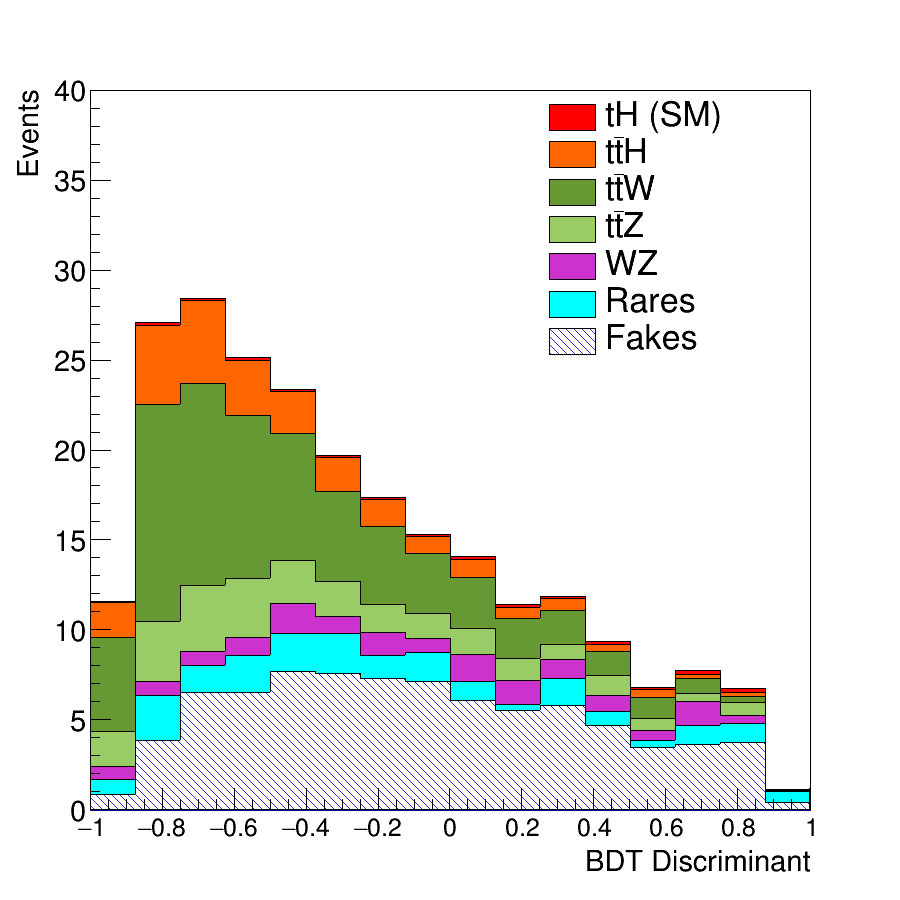
\includegraphics[width=\textwidth]{Chapter3/kos.png}
	\end{minipage}
	\hfill
	\begin{minipage}[b]{0.48\textwidth}
		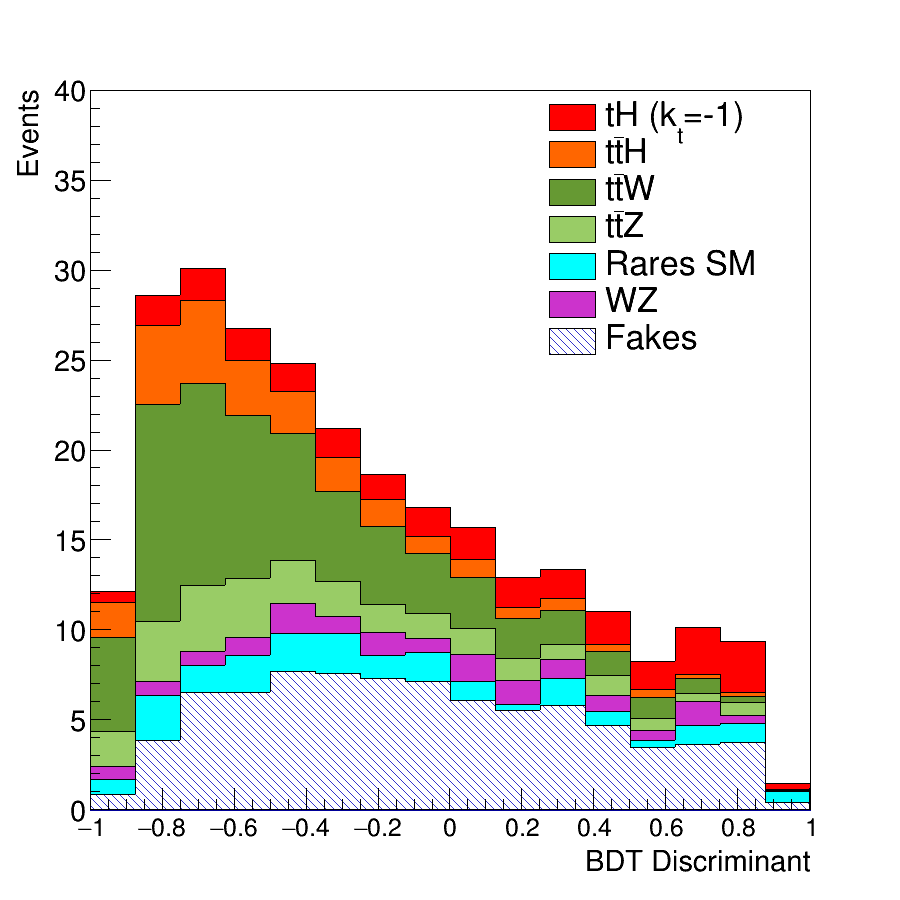
\includegraphics[width=\textwidth]{Chapter3/kos2.png}
	\end{minipage}
\caption{Distribution of BDT discriminant for signal and background in the case of SM (left) and inverted coupling scenario (right) \cite{th1}}
\label{bdt2}
\end{figure}


	\chapter{Statistical Analysis}
To estimate the sensibility of the $tH$ signal, we define an Asimov dataset, made by replacing the ensemble of simulated backgrounds and signal by a single one. The statistical uncertainty of the Asimov data is calculated as $\sqrt{n}$, with $n$ the number of events. The uncertainty of the signal strength is estimated by applying a  fit to the Asimov dataset, where the model
is constructed from the sum of the individual backgrounds and signal. The fit is implemented using a Poisson likelihood and gaussian constraints for the systematical uncertainties in the model.


\section{Likelihood and fit procedure}
The likelihood function is the product of Poisson probabilities for all bins of the BDT distribution. The likelihood function has the form
\begin{align}
L(\mu,\alpha)=\prod_{j=1}^{N}\frac{(\mu s_j +b_j)^{n_j}}{n_j !}e^{-(\mu s_j+b_j)} \prod_{k=1}^M e^{\frac{-\alpha^2_k}{2}}
\end{align}
where $N$ is the total number of bins, n is the number of events in a bin $j$,  $s_j$ is the number of signal events, $\mu$ is the parameter of signal strength and  $b_j$ is the number of background events.
$b_j$ is the sum of different background processes $k$
\begin{align}
b_j=\sum_k b_j^k(1+\sigma_k \alpha)
\end{align}
$\alpha$ is the parameter that modifies the expected background prediction and $\sigma_k$ is the systematic uncertainty of the associated background. \\

The fit is applied by minimizing the $-\log{L}$ (NLL) with respect to the parameter $\mu$ and $\alpha_k$. The minimization is performed by using the package ROOFIT \cite{roofit}.
%log es usado para evitar valores extremadamente pequenos debido a los productos de los exponenciales
%negativo es para hacer una minimizacion, positivo es maximizacion
\pagebreak

\begin{table}[ht!]
	\centering
	\caption{Postfit for each yield.Prefit uncertainty is statistical only. Postfit uncertainty is statistical + systematic.}
\begin{tabular}{ccc}
	\hline
	Process  & SM    & $k_t=-1$ \\
	\hline
$t\bar{t}W$  &  68$\pm$8.9& 68 $\pm$8.9 \\
	$t\bar{t}Z$  & 25.9$\pm$3.8&25.9$\pm$3.8\\
$WZ$ &  15.1$\pm$7.4& 15.1$\pm$7.4\\
Rares &  20.8$\pm$4.8& 20.8$\pm$4.8 \\
	Fakes  &  80.9$\pm$9.0&  80.9$\pm$8.9 \\
	$t\bar{t}H$  &   24.2$\pm$2.0 &  24.2$\pm$2.0 \\
\hline
$tH$&  2.14$\pm$16.56 &26.22$\pm$13.11 
\end{tabular}
\label{table1}
\end{table}

In the figure \ref{simple} and table \ref{table1} , shows the results of the model fitting using the Asimov data for both models. As mentioned before, the  $k_t=-1$, the number of events for the $tH$ signal is more than ten times, compared to SM. This causes that the fit model have access to more data, and so improve the fit a bit. Due to low $tH$ number of events, the uncertainty after the fit is big, compared to the $k_t=-1$ model, where the uncertainty is around 50$\%$. Because of the model, the values of the backgrounds don't change.
\begin{figure}[!htbp]
	\centering
	\begin{minipage}[b]{0.48\textwidth}
		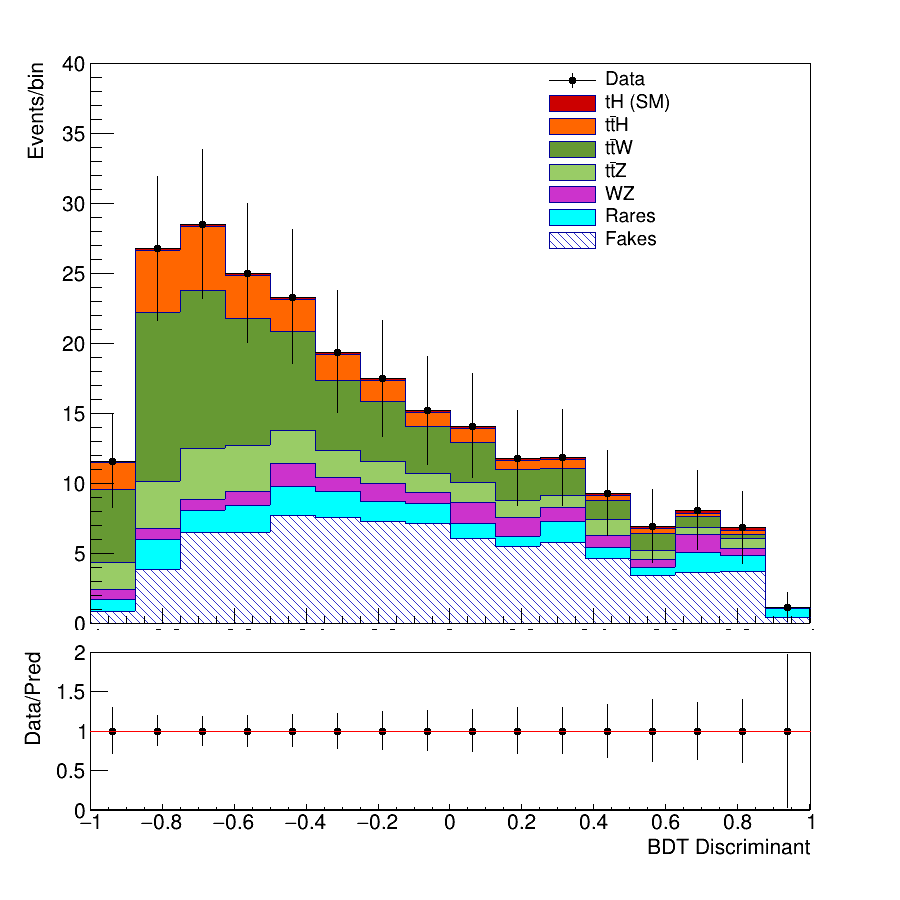
\includegraphics[width=\textwidth]{Chapter4/simple.png}
	\end{minipage}
	\hfill
	\begin{minipage}[b]{0.48\textwidth}
		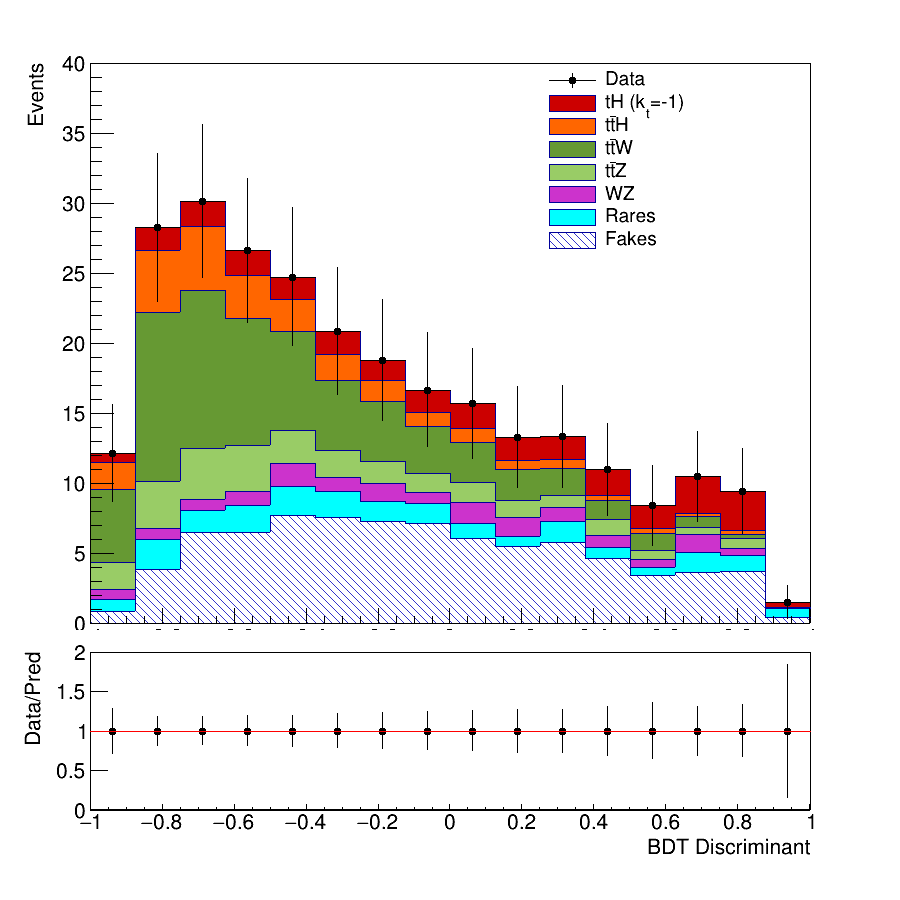
\includegraphics[width=\textwidth]{Chapter4/simple-kt-1.png}
	\end{minipage}
	\caption{Post fit signal and background yields for tH process for SM (Left) and $k_t=-1$ (Right).
		In the box below each distribution, the ratio of the observed and predicted event yields is shown}
\label{simple}
\end{figure}
In the table \ref{parameters}, shows the $\mu$ and $\alpha$ parameters. For the pre-fit, values of $\alpha$ are set to zero and $\mu$ is set to 1.After the fit,  $\alpha$ parameters set to zero indicates that in the fit, the values of the backgrounds didn't changed for the SM and the $\mu$ parameter set to 1 indicates that the signal strength also didn't changed, but its uncertainty is also big.
However, in the model $k_t=-1$, the $\alpha$ parameters shows a slightly change, that indicates changes in the backgrounds, but with a great uncertainty. For the $\mu$, it shows the same size, but the uncertainty is estimated to be 50$\%$, corresponding to the results obtained for the events yields.
\begin{table}[ht]
	\centering
	\caption{$\alpha$ and $\mu$ values for 35.9 fb$^{-1}$}
	\begin{tabular}{ccc}
		\hline
		Parameter  & SM &kt\\
		$\mu$   & 1.00 $\pm$  7.74& 1.0 $\pm$  0.5\\
		$alpha_ttw$&  0.00 $\pm$  0.89&  6.32$\times 10^{-09}$ $\pm$  089\\
		$alpha_ttz$ &  0.00 $\pm$  0.98& 1.90$\times 10^{-09}$ $\pm$  0.98\\
		$alpha_wz$   & 0.00 $\pm$  0.97& -5.33$\times 10^{-09}$9 $\pm$  0.97\\
		$alpha_tz$   &0.00 $\pm$  0.95&-7.83$\times 10^{-09}$ $\pm$  0.98 \\
		$alpha_fakes$ &   0.00 $\pm$  0.96&  3.47 $\times 10^{-09}$ $\pm$  0.95\\
		$alpha_tth$ &0.00 $\pm$  0.98& 2.61$\times 10^{-09}$ $\pm$ 0.98\\
	\end{tabular}
\label{parameters}
\end{table}

For the analysis of the likelihood function,  we take likelihood ratio
\begin{align}
	\lambda(\mu,\theta(\mu))=\frac{L(\mu,\hat{\hat{\theta}}(\mu))}{L(\hat{\mu},\hat{\theta}(\mu))}
\end{align}
Where $\hat{\hat{\theta}}(\mu) $ in the numerator denotes the value of $\theta(\mu)$ that maximizes L for the specified $\mu$, that is , the conditional maximum-likelihood (ML) estimator of $\hat{\theta}(\mu)$ 
The denominator represents the  maximized  likelihood function, where $\hat{\mu}$ and $\hat{\theta}$ are
their ML estimators.
The presence of the nuisance parameters broadens the profile likelihood as a
function of $\mu$ relative to what one would have if their values were fixed. This reflects the loss
of information about $\mu$ due to the systematic uncertainties

\section{Limit calculation}
Due to the large background, the signal strength for the Asimov data with 35.9 $fb^{-1}$ is consistency with zero.
Therefore, we estimate an upper limit on the signal strenght at 95 $\%$ level of confidence.








For purposes of establishing an upper limit on the strength parameter $\mu$ , we consider two
closely related test statistics. First, we may define
\begin{align}
q_{\mu}=  \Big\{    \begin{array}{ll}
-2\ln\lambda(\mu) \qquad \hat{\mu} \leq \mu	\\
0  \qquad \qquad \qquad \hat{\mu}< 0
\end{array}
\end{align}
The reason for setting $q_\mu = 0$
for $\hat{\mu}>\mu $ is that when setting an upper limit, one would not regard data with $\hat{\mu}>\mu $ as
representing less compatibility with $\mu$ than the data obtained, and therefore this is not taken
as part of the rejection region of the test. From the definition of the test statistic one sees that
higher values of $q_\mu$ represent greater incompatibility between the data and the hypothesized
value of $\mu$.



\begin{table}[ht!]
	\caption{Estimation of $\mu$ and upper limits  for extrapolations}
	\begin{tabular}{|c|c|c|c|c|}
		\hline
		Luminosity (fb$^{-1}$)	&$\mu$ &$\mu$ for $k_t=-1$ &$\mu$ upper limit &$\mu$ upper limit for $k_t=-1$ \\
		\hline
		35.9 & 1.00 $\pm$  8.32 & 1.00 $\pm$  0.249&	22.328 & 2.777   \\
		\hline
		150& 1.00 $\pm$  6.44 & 1.00 $\pm$  0.544  &12.619 &0.915 \\
		\hline
		300&1.00 $\pm$  4.83 &1.00 $\pm$  0.407 & 9.427&0.649 \\
		\hline
		3000&1.00 $\pm$  1.54 & 1.00 $\pm$  0.151&	 3.442 & 0.25
		\\
		\hline
	\end{tabular}
\end{table}



	\chapter{Conclusion and outlook}


	
	% ********************************** Back Matter *******************************
	% Backmatter should be commented out, if you are using appendices after References
	%\backmatter
	
	% ********************************** Bibliography ******************************
	\begin{spacing}{0.9}
		
		% To use the conventional natbib style referencing
		% Bibliography style previews: http://nodonn.tipido.net/bibstyle.php
		% Reference styles: http://sites.stat.psu.edu/~surajit/present/bib.htm
		
		%\bibliographystyle{acm}
		\bibliographystyle{unsrtnat} % Use for unsorted references  
	%	\bibliographystyle{plainnat} % use this to have URLs listed in References
		\cleardoublepage
		\bibliography{References/references} % Path to your References.bib file
		
		
		% If you would like to use BibLaTeX for your references, pass `custombib' as
		% an option in the document class. The location of 'reference.bib' should be
		% specified in the preamble.tex file in the custombib section.
		% Comment out the lines related to natbib above and uncomment the following line.
		
		%\printbibliography[heading=bibintoc, title={References}]
		
		
	\end{spacing}
	
	% ********************************** Appendices ********************************
	
	\begin{appendices} % Using appendices environment for more functunality
		
	%	%!TEX root = ../thesis.tex
% ******************************* Thesis Appendix A ****************************
\chapter{Values for \protect \texorpdfstring{$\alpha$ and $\mu$}{and}}
\begin{verbatim}
Floating Parameter		\qquad		FinalValue +/- Error \\
$---------------------------------$			\\
Lumi \quad	\qquad	\qquad		\qquad		1.0082e+00 +/-  2.42e-02\\
alpha\_sample\_tth\_sys	\quad	1.9100e-01 +/-  9.94e-01\\
alpha\_sample\_ttw\_sys	\quad	8.7537e-01 +/-  9.18e-01\\
alpha\_sample\_ttz\_sys	\quad	2.0012e-01 +/-  9.95e-01\\
alpha\_sample\_tz\_sys\qquad	1.6749e-01 +/-  1.00e+00\\
alpha\_sample\_wz\_sys\qquad	 1.2732e-01 +/-  9.84e-01 \\
alpha\_sample\_fakes\_sys	4.5030e-01 +/-  7.17e-01\\
mu 	\qquad	\qquad	\qquad	\qquad	\qquad	2.4975e+00 +/-  1.29e+01
\end{verbatim}


\begin{verbatim}
Floating Parameter			\qquad		FinalValue +/- Error \\
$-----------------------------$
Lumi \quad	\qquad	\qquad		\qquad	\qquad 1.0085e+00 +/-  2.40e-02\\
alpha\_sample\_tth\_sys	\quad	1.9290e-01 +/-  1.00e+00 \\
alpha\_sample\_ttw\_sys	\quad	8.7911e-01 +/-  9.42e-01\\
alpha\_sample\_ttz\_sys	\quad	2.0370e-01 +/-  9.94e-01\\
alpha\_sample\_tz\_sys\qquad	1.8269e-01 +/-  9.69e-01\\
alpha\_sample\_wz\_sys\qquad	1.4244e-01 +/-  9.99e-01\\
alpha\_sample\_fakes\_sys	1.4243e-01 +/-  9.98e-01\\
mu \qquad	\qquad	\qquad	\qquad	\qquad 6.9361e-02 +/-  1.02e+00
\end{verbatim}
	%	%!TEX root = ../thesis.tex
% ******************************* Thesis Appendix B ********************************

\chapter{Scattering and cross section}
In classical mechanics, scattering is  a set of particles which deviate from their original trajectory to one or many ways. Examples of scattering are particle collisions and particles that deviates in a potential field.\\  
The cross section in a scattering is the area transverse to the relative motion between two object to scatter from each other.\cite{goldstein}
For a particle which deviates from its original way due to a potential whose center is at rest, the scattering angle is given by
\begin{align}
    \theta =\pi - 2\phi_0
\end{align}
with 
\begin{align}\label{sc1}
\phi_0 = \int_{r_0}^\infty \frac{M/r^2 d r}{\sqrt{2m(E-U(r)-M^2/r^2}}
\end{align}
with $r_0$ the nearest position to the center of potential and $U(r)$ is the potential. Now for great velocity , if we change $E=\frac{1}{2}mv^2$ and  $M=mpv$ and substitute in \ref{sc1}, we have \begin{align}
    \phi_0 = \int_{r_0}^\infty \frac{\rho /r^2 d r}{\sqrt{1-\frac{\rho^2}{r^2}-2U(r)/mv^2}}
\end{align} 
in terms of parameter of impact $\rho$ and the position\cite{landau}.
\begin{figure}[ht!] 
    \centering
    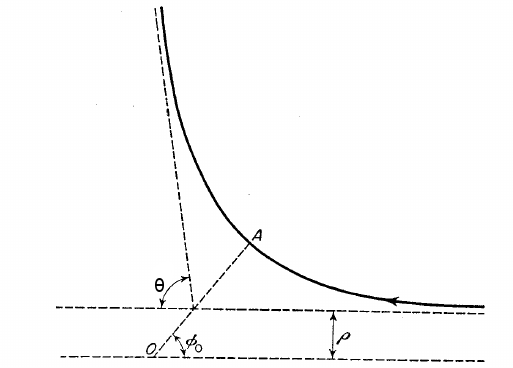
\includegraphics[scale=0.8]{Chapter1/sc.png}
    \caption{Diagram of scattering for a particle in a potential field\cite{landau}}
    \label{sc2}
\end{figure}
In a scattering of a beam of identical particles with velocity of $v$ , let $dN$ the number of particles scattered per unit of time through the angles $\theta$ and $\theta +d\theta$
The effective cross section is 
\begin{align}
    d\sigma=\frac{dN}{n}
\end{align}
n represents the number of particles passing in unit of time in a unit area of beam cross section. If $\rho$ is $\theta$ dependient, then the effective cross section is 
\begin{align}
    dN=2\phi \rho n d\rho \qquad d\sigma=2\phi \rho d\rho
\end{align}
rewriting $d\sigma$

\begin{align}
    d\sigma=2\phi \rho \left| \frac{d\rho}{d\theta} \right| d\theta
\end{align}
the derivative $\frac{d\rho}{d\theta}$ can be negative ,so it is necessary the modulus \cite{landau}. In a three dimension model, $d\sigma$ is related to the solid angle, instead of $d\theta$ , so the solid angle between the angles $\theta$ and $\theta+d\theta$ is
\begin{align}
    d\Omega=2\pi \sin{\theta}d\theta
\end{align}
thus, the cross section is 
\begin{align}
     d\sigma=   \frac{\rho(\theta)}{\sin{\theta}} \left| \frac{d\rho}{d\theta} \right| d\Omega
\end{align}
\begin{figure}[!htbp]
\centering
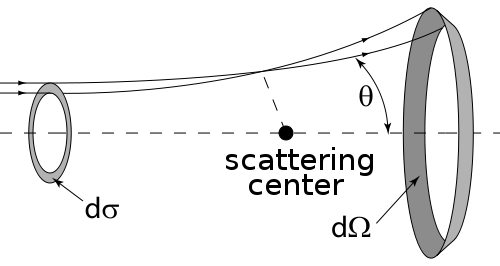
\includegraphics[scale=0.7]{Chapter1/cs1.png}
 \caption{Drawing of an idealized scattering process showing the differential solid angle $\Delta\Omega$ and the
scattering angle $\theta$ \cite{gross} }
\label{sc}
\end{figure}

let N be the number of events. In terms of of solid angle
\begin{align}
    dN=\text{L} d\sigma=\text{L} \frac{d\sigma}{d\Omega} d\Omega \qquad \frac{d\sigma}{d\Omega}=\frac{dN}{\text{L}d\Omega}
\end{align}
For a collision of two particles that produce many particles, the cross section is given by 
\begin{align}\label{sc3}
\sigma=\frac{S\hbar^2 }{4\sqrt{(p_1 \cdot p_2)^2 -(m_1 m_2 c^2)^2} }\int \left| M \right|^2 (2\pi)^4 \delta^4(p_1-p_2-...p_n)\times \prod_{j=2}^n 2\pi \delta (p_j^2-m_j^2 c^2)\theta (p_j^0)\frac{d^4 p_j}{(2\pi)^4}
\end{align} 
the structure of the equation \ref{sc3} is similar to the equation \ref{dm}\cite{griff}.\\

Experimentally
\begin{align}
d\sigma=\frac{\text{number of particles scattered into solid angle} \Delta\Omega}{\text{(number of particles incident)(scattering centers/area)}}
\end{align}
		
	\end{appendices}
	
	% *************************************** Index ********************************
	\printthesisindex % If index is present
	
\end{document}
